\documentclass{article}
\usepackage[utf8]{inputenc}
\usepackage[italian]{babel}
\usepackage{amsmath}
\usepackage{amssymb}
\usepackage{siunitx}
\usepackage{tabularray}
\usepackage{graphicx}
\usepackage{float}
\usepackage{minted}
\usepackage[page]{appendix}
\newcommand*{\diam}{\varnothing}
\newcommand*{\best}[1]{{#1}_\text{best}}
\newcommand*{\bestp}[1]{{\left(#1\right)}_\text{best}}
\newcommand*{\pbest}[1]{\left({#1}_\text{best}\right)}
\newcommand*{\pbestp}[1]{\left({\left(#1\right)}_\text{best}\right)}
\newcommand*{\errrel}[1]{\frac{\delta #1}{{#1}_\text{best}}}
\newcommand*{\Th}{^{232}_{\;\;90} \text{Th}}
\title{
    Laboratorio di Fisica 1\\
    R4: Misura di variabili aleatorie
}
\author{Gruppo 17: Bergamaschi Riccardo, Graiani Elia, Moglia Simone}
\date{8/11/2023 – 15/11/2023}
\makeindex
\begin{document}

\maketitle

\begin{abstract}
    Il gruppo di lavoro ha misurato due variabili aleatorie, osservando come queste
    rispecchino le rispettive distribuzioni teoriche (di Bernoulli e di Poisson).
\end{abstract}

\section{Processo di Bernoulli}

\subsection{Dati sperimentali}
Eseguiamo 400 lanci di sei dadi distinti\footnote{Li distinguiamo in base al colore},
registrandone tutti i risultati.
Per ogni possibile risultato $s\in\left[1;6\right]\cap\mathbb{N}$, possiamo così
definire una variabile aleatoria\footnote{\emph{Notazione.} Per noi $0\in\mathbb{N}$.}
$x_s\in\left[0;6\right]\cap\mathbb{N}$ come il
numero di dadi, fra i sei lanciati, con risultato pari ad $s$.
Possiamo considerare il lancio dei sei dadi come un processo di Bernoulli,
in quanto i risultati dei dadi sono indipendenti fra loro. Di conseguenza,
la distribuzione di probabilità di $x_s$ è data da:
\[
    p \left(x_s=k\right) =
        \binom{6}{k}
        \left(\frac{1}{6}\right)^k
        \left(\frac{5}{6}\right)^{6-k}
        \qquad\forall k\in\left[0;6\right]\cap\mathbb{N}
\]
Di seguito riportiamo gli istogrammi dei dati così raccolti, assieme ai valori attesi,
calcolati mediante la distribuzione teorica.

\begin{center}
    \begin{figure}[H]
        % trim={< v > ^}
        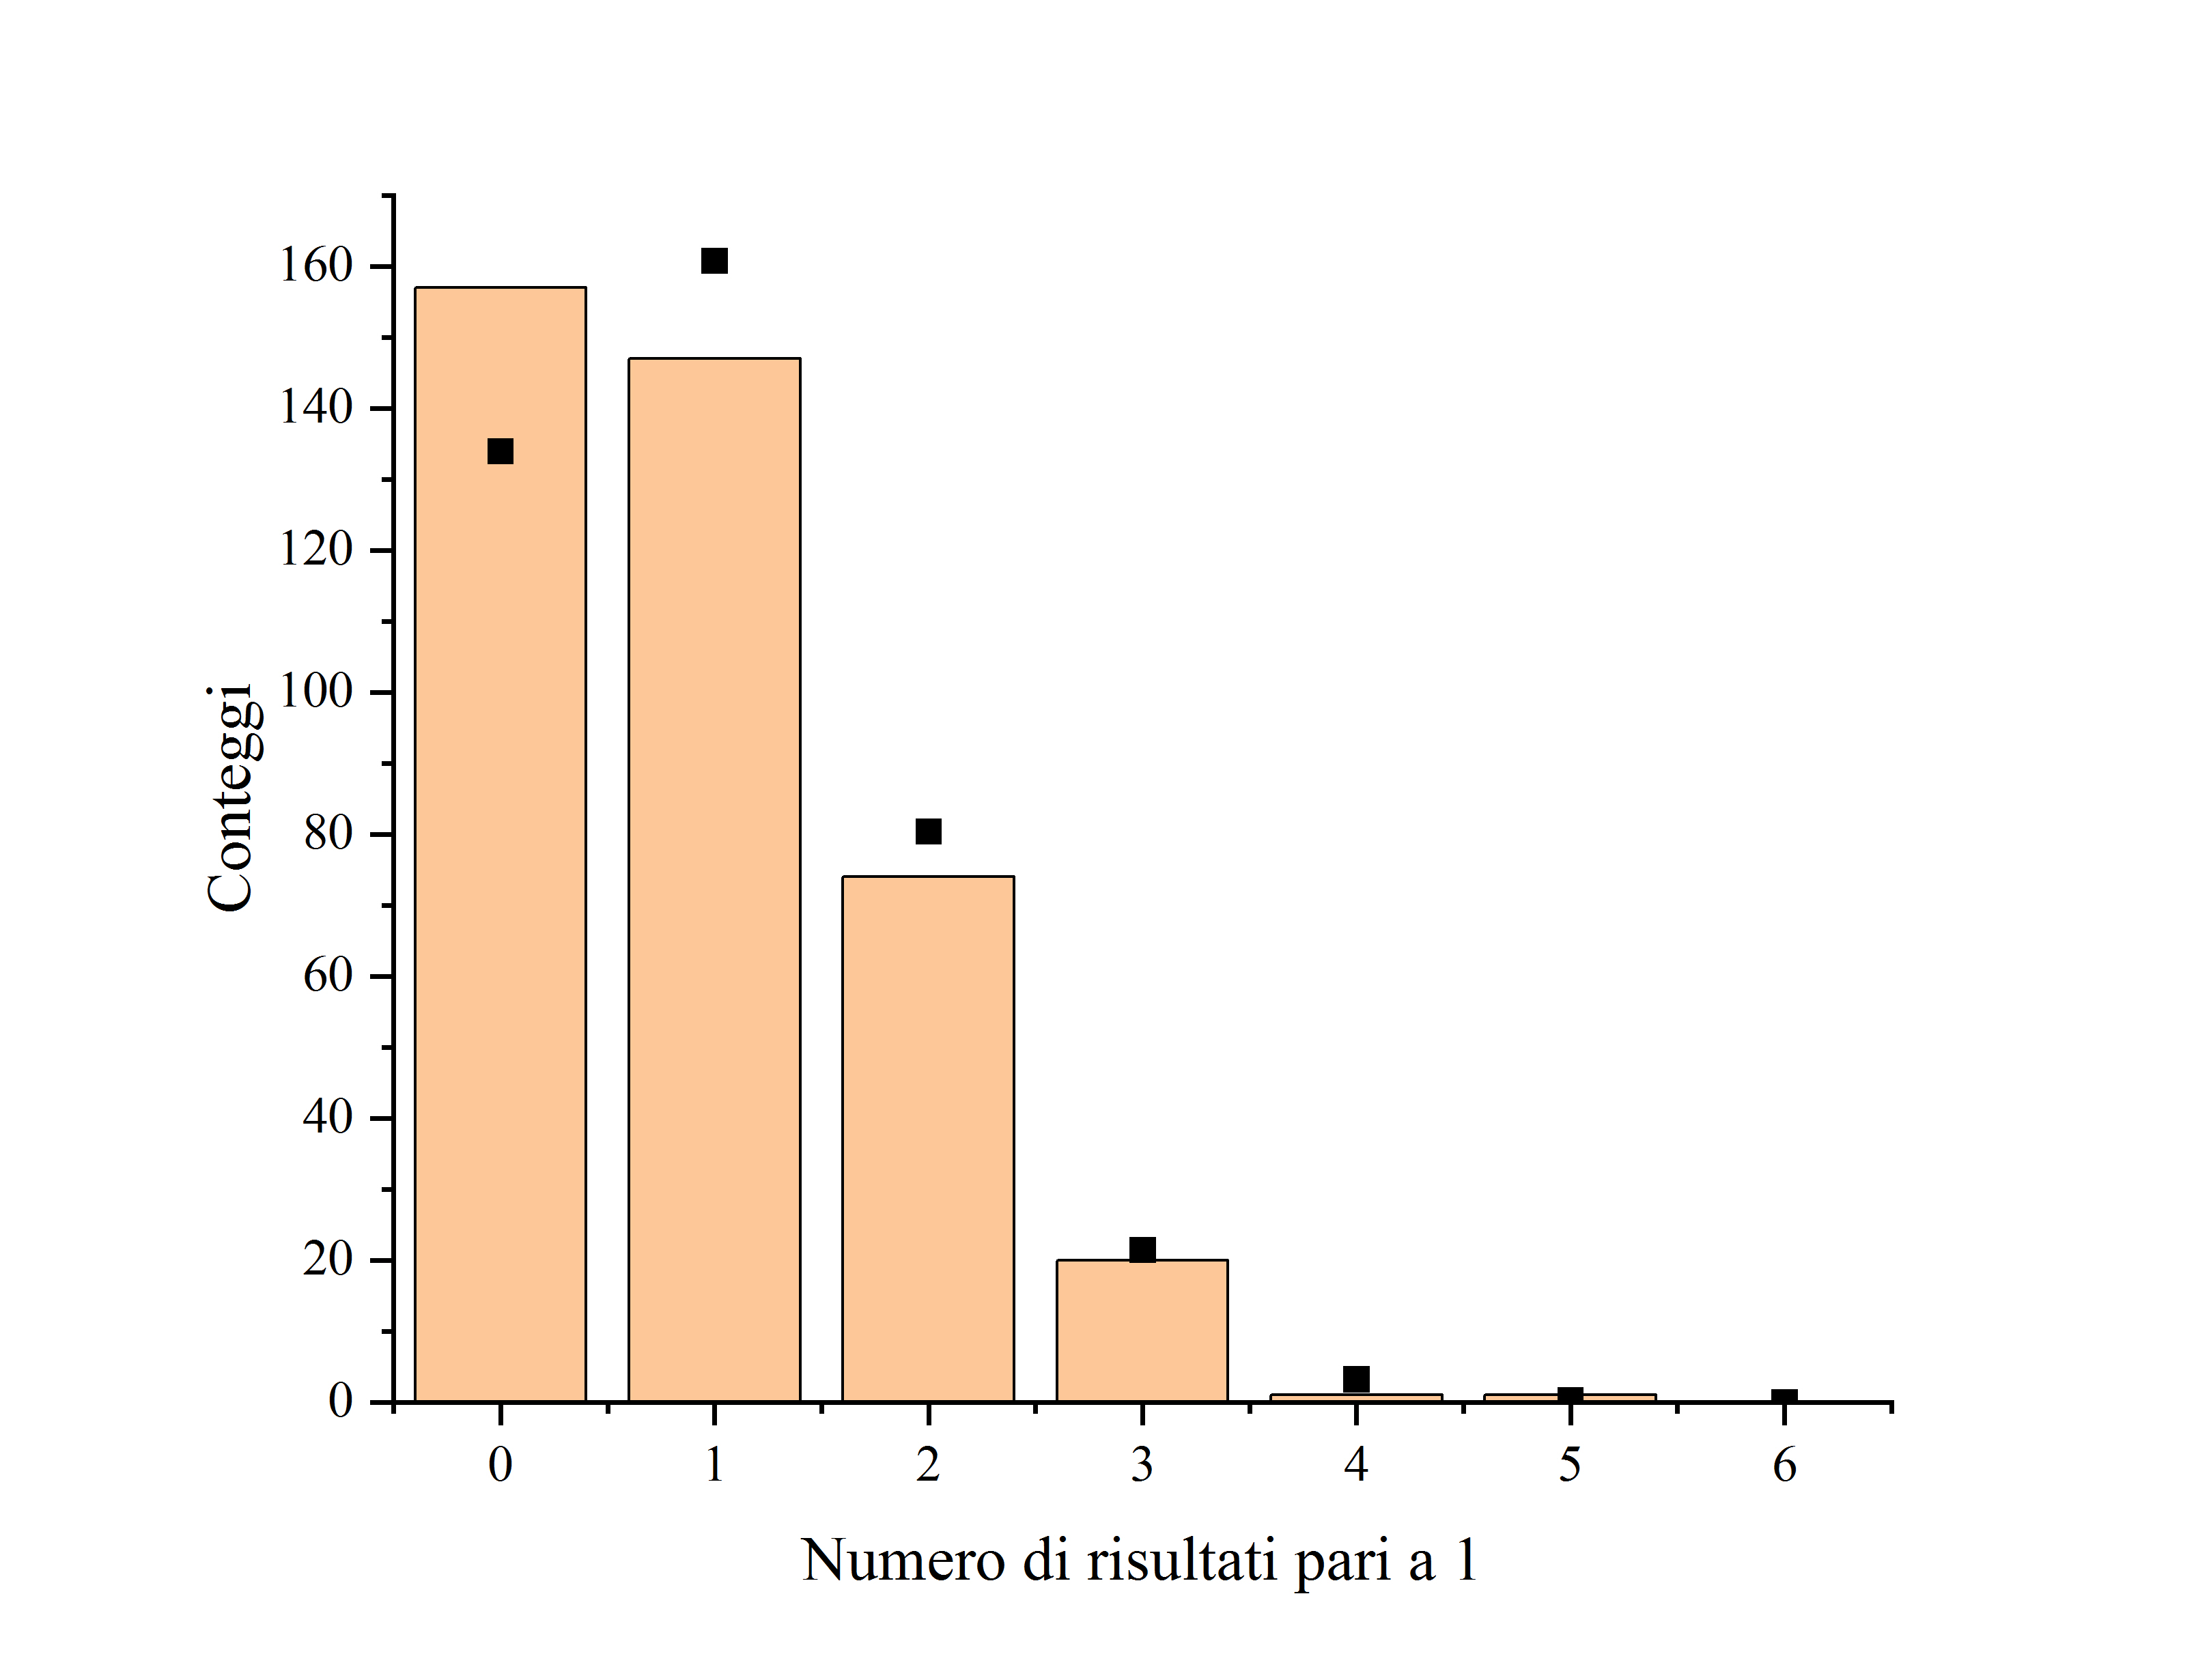
\includegraphics[trim={2cm .5cm 2.4cm 2.1cm},clip,width=.5\textwidth]{img/Dadi1.jpg}
        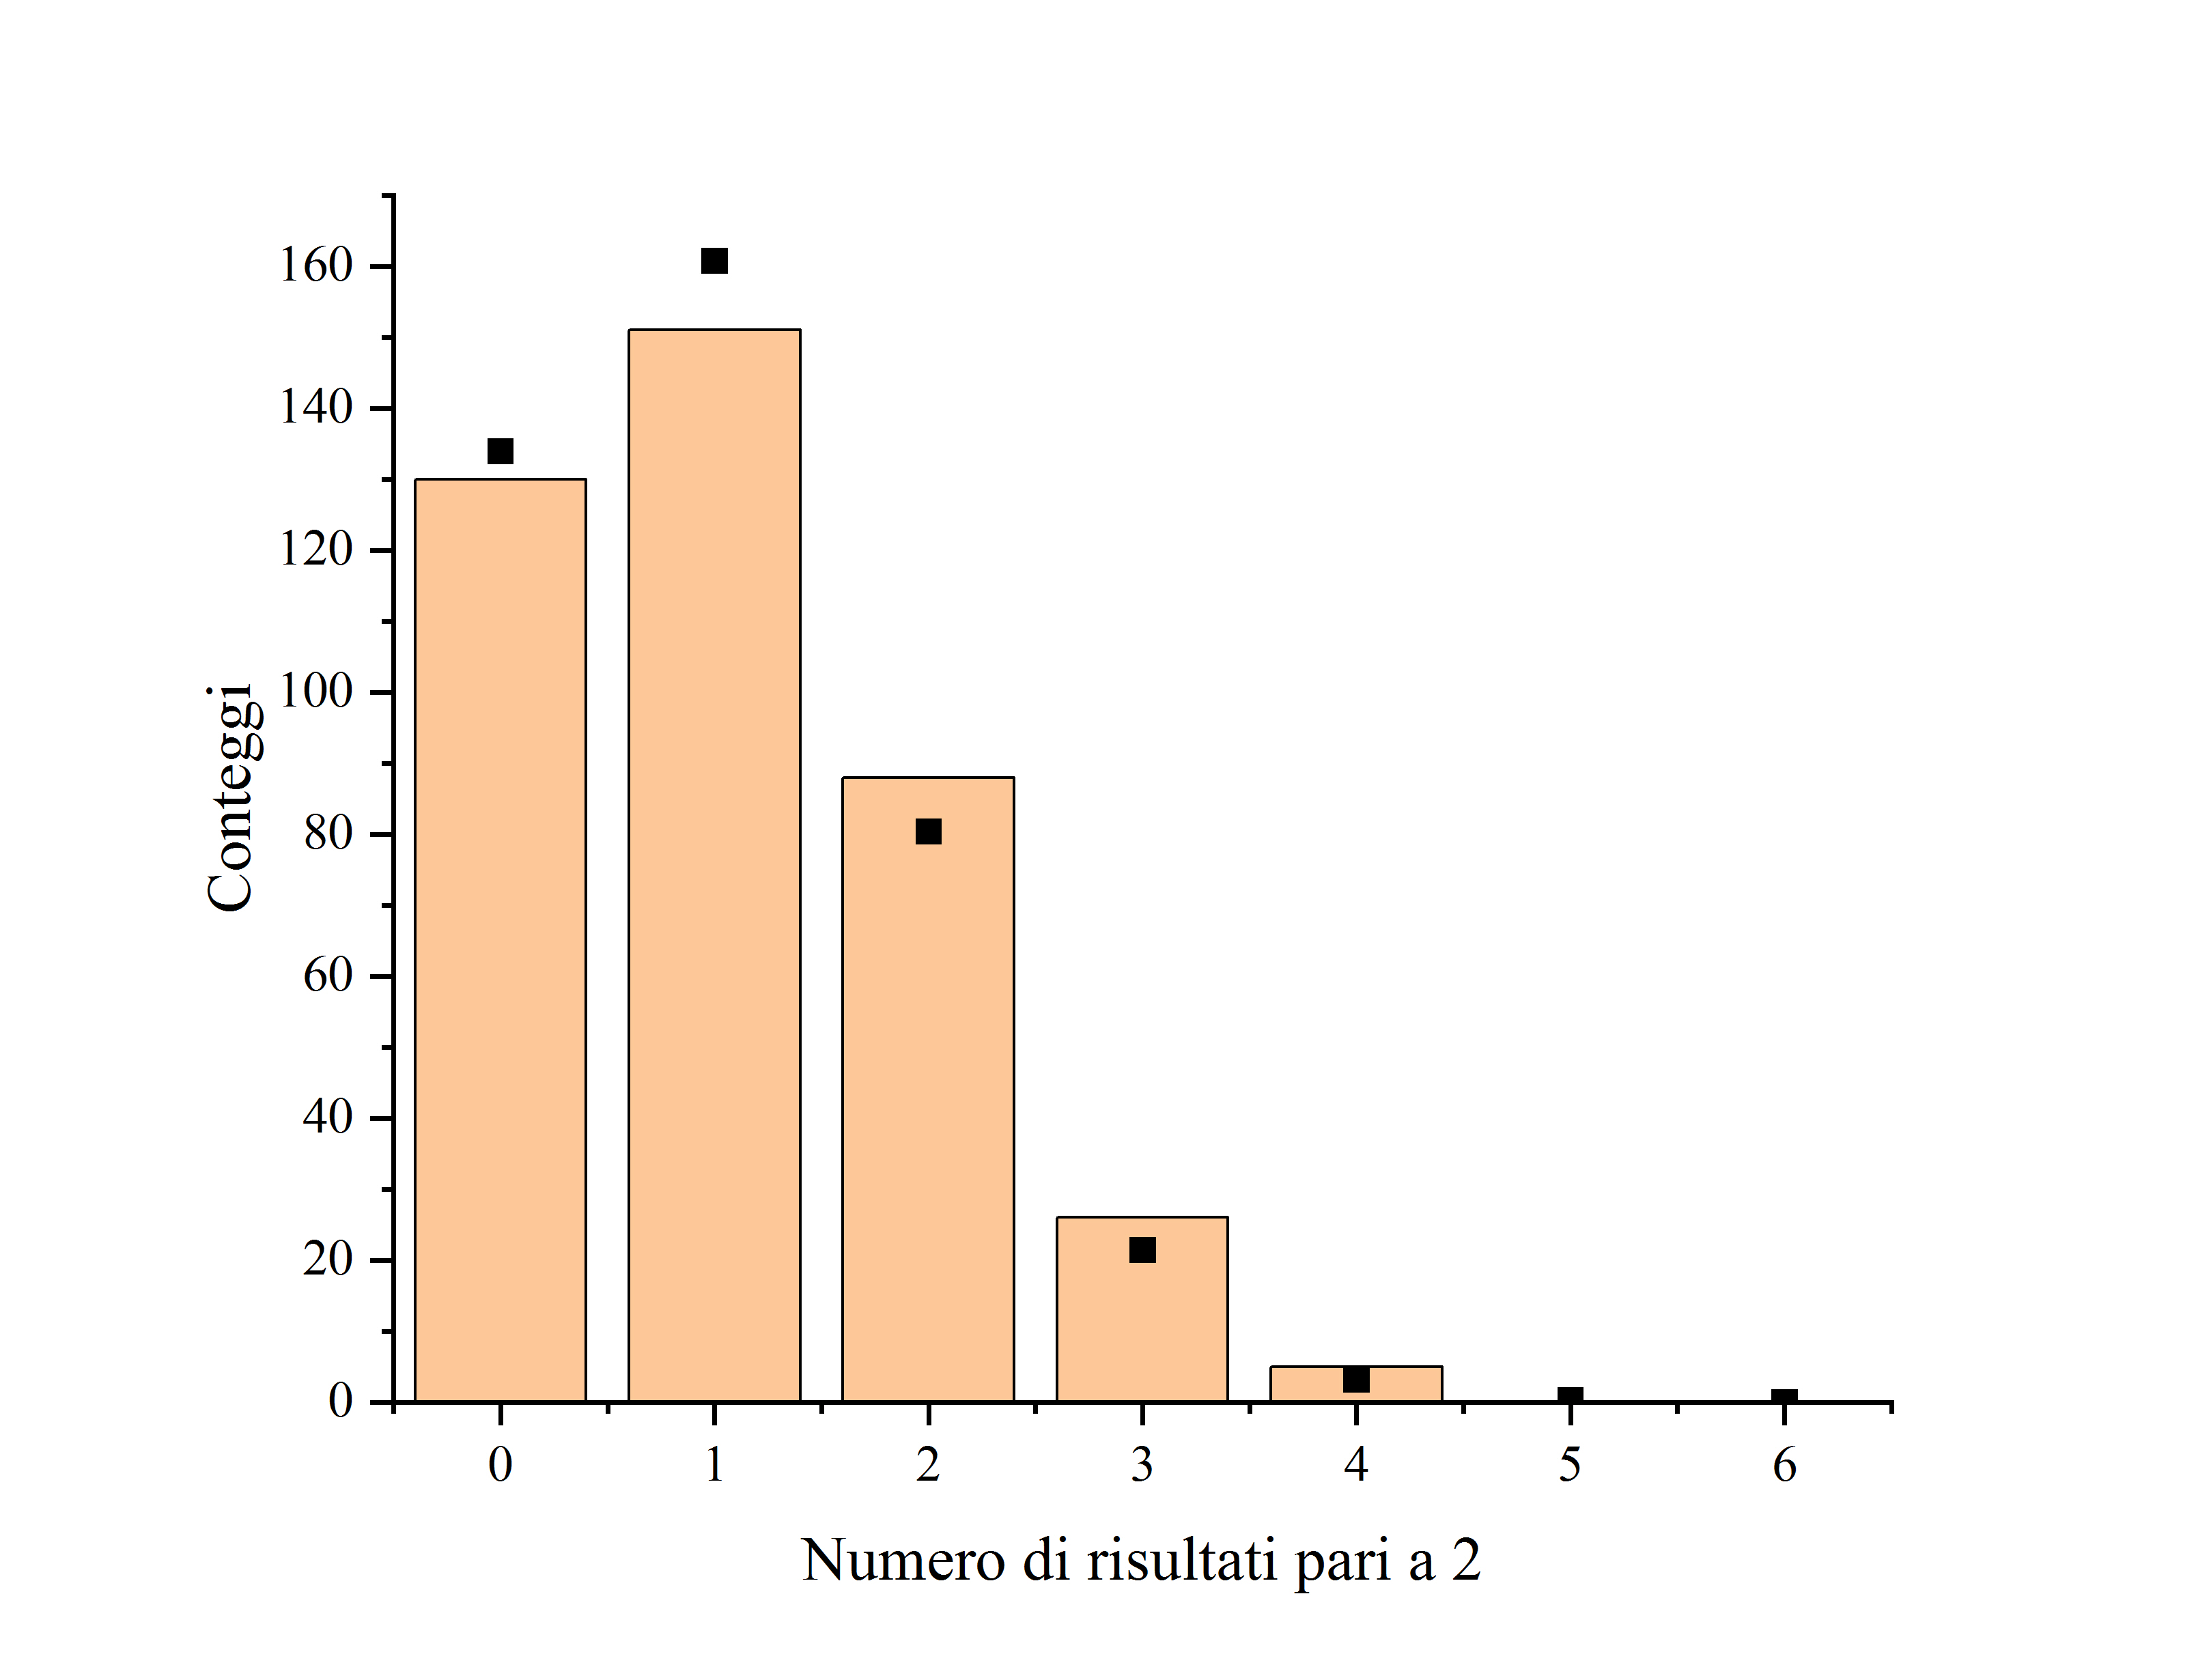
\includegraphics[trim={2cm .5cm 2.4cm 2.1cm},clip,width=.5\textwidth]{img/Dadi2.jpg}
        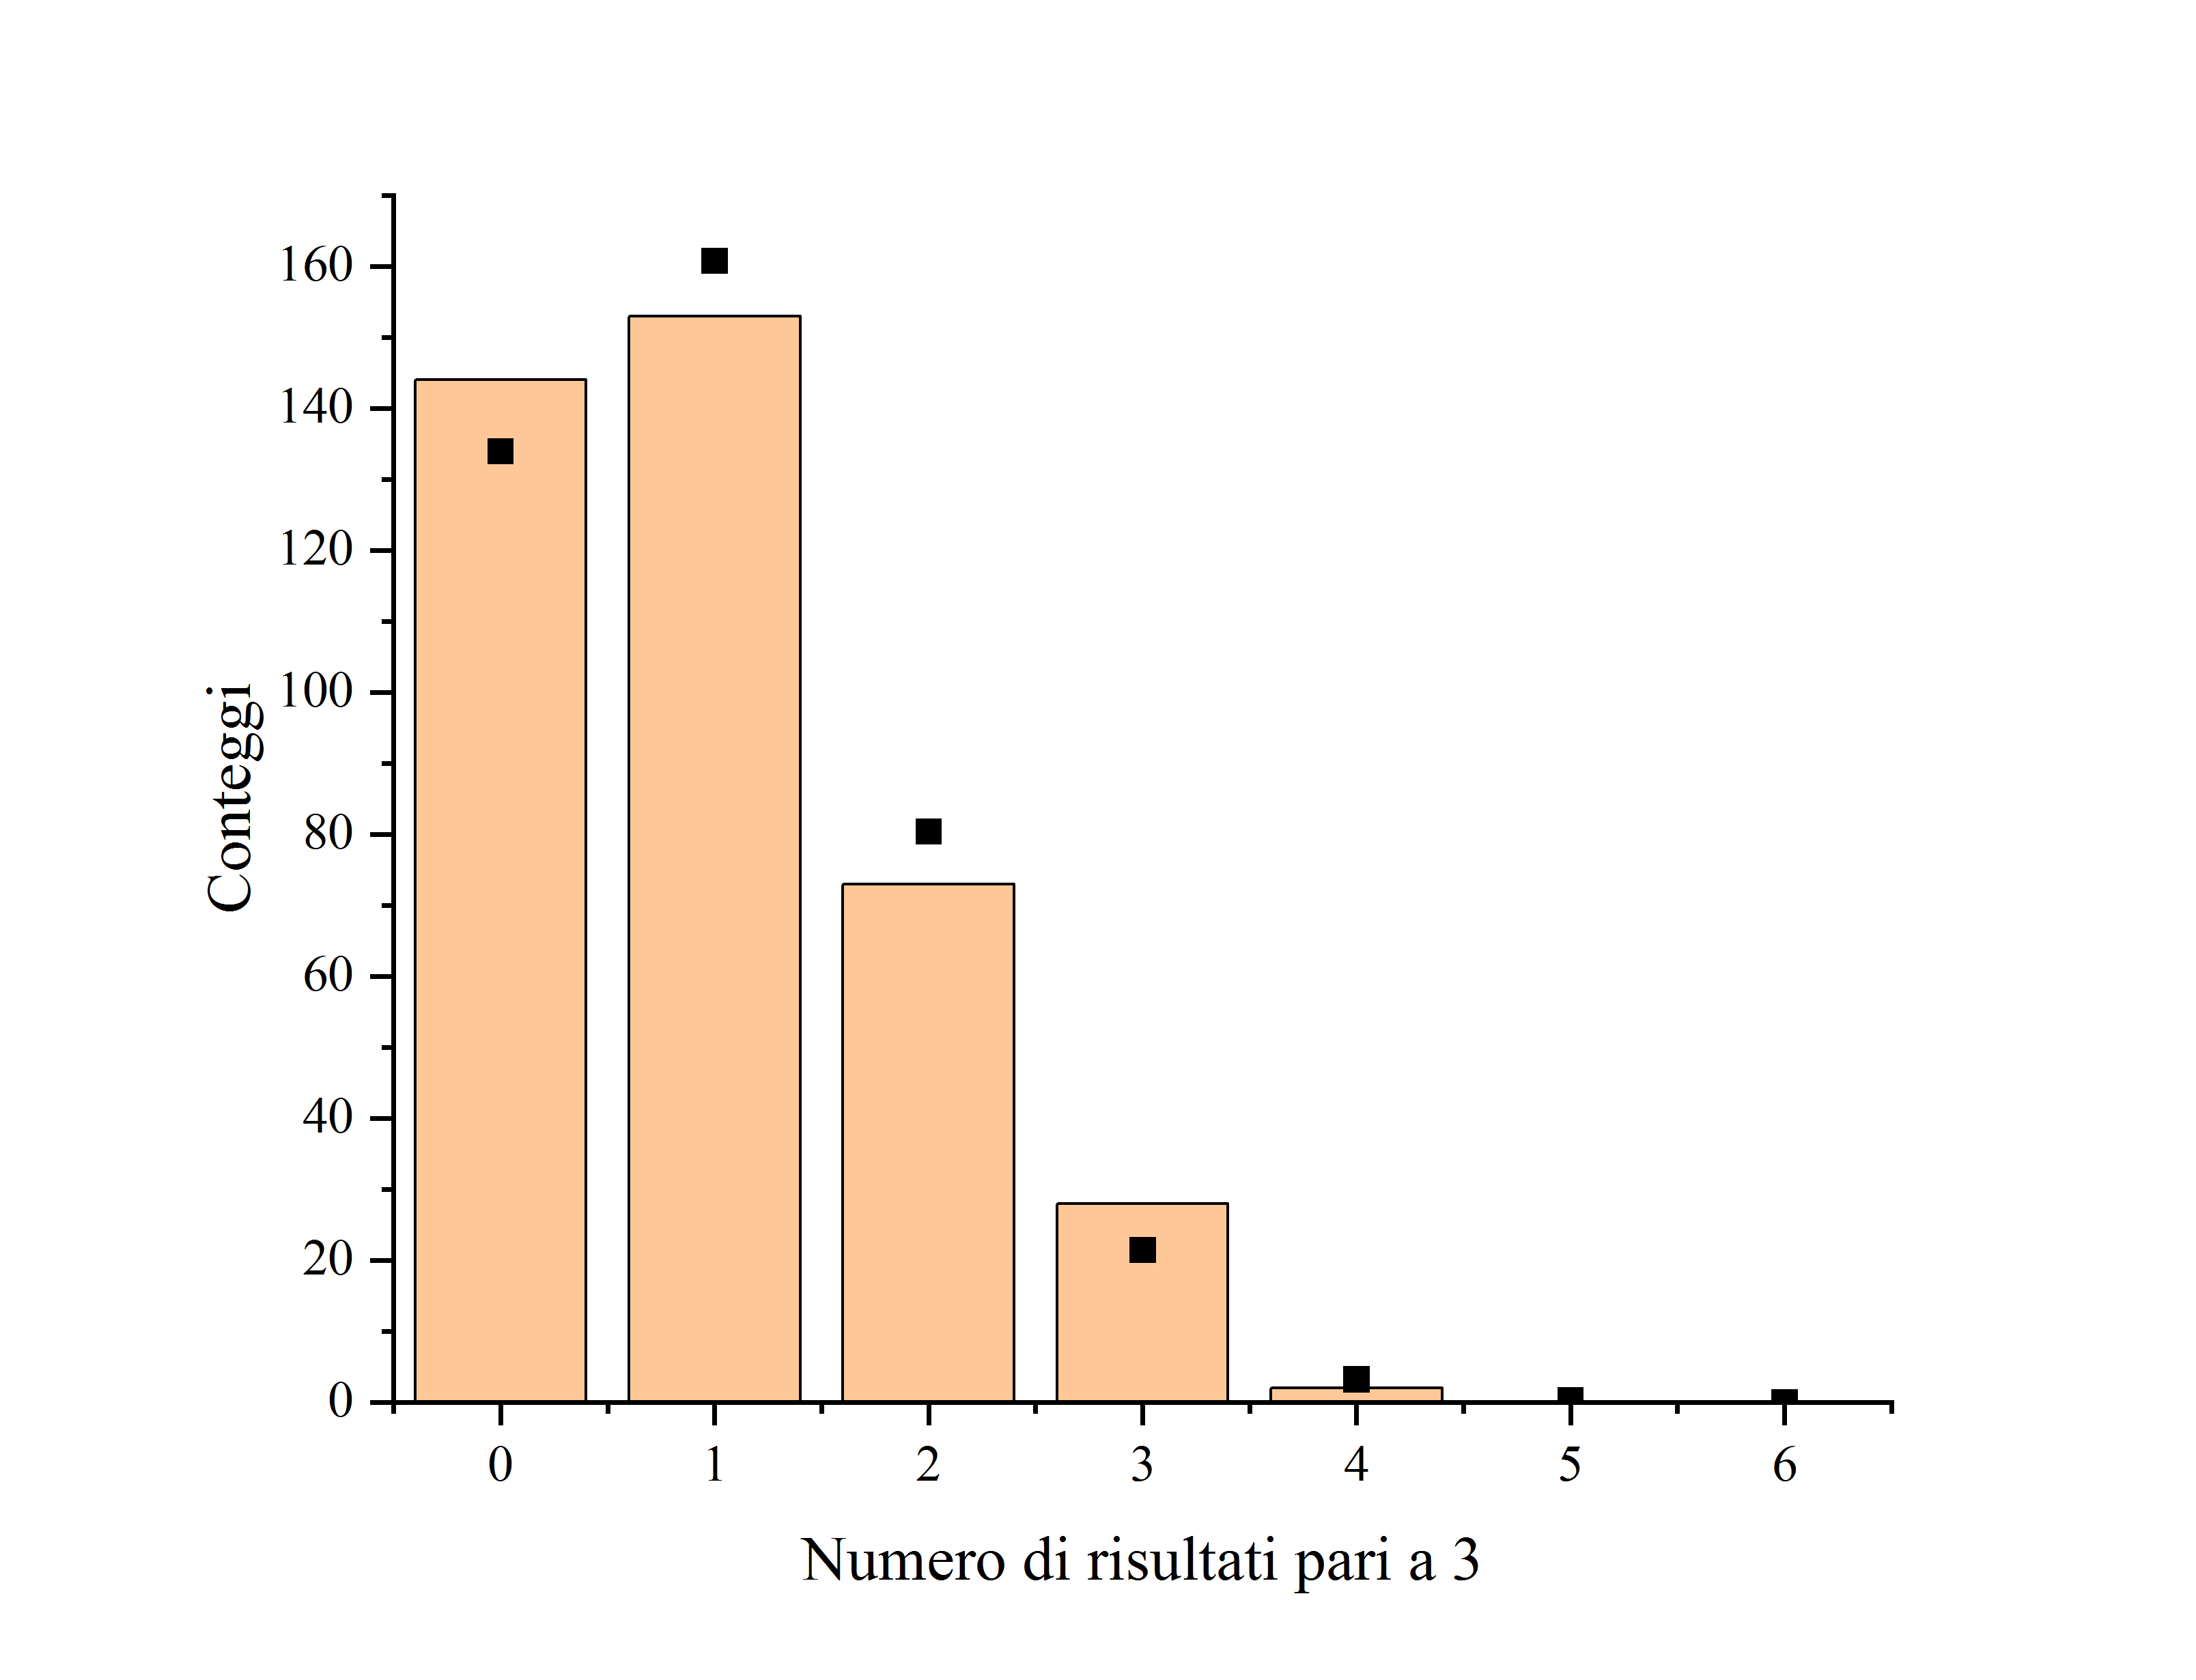
\includegraphics[trim={2cm .5cm 2.4cm 2.1cm},clip,width=.5\textwidth]{img/Dadi3.jpg}
        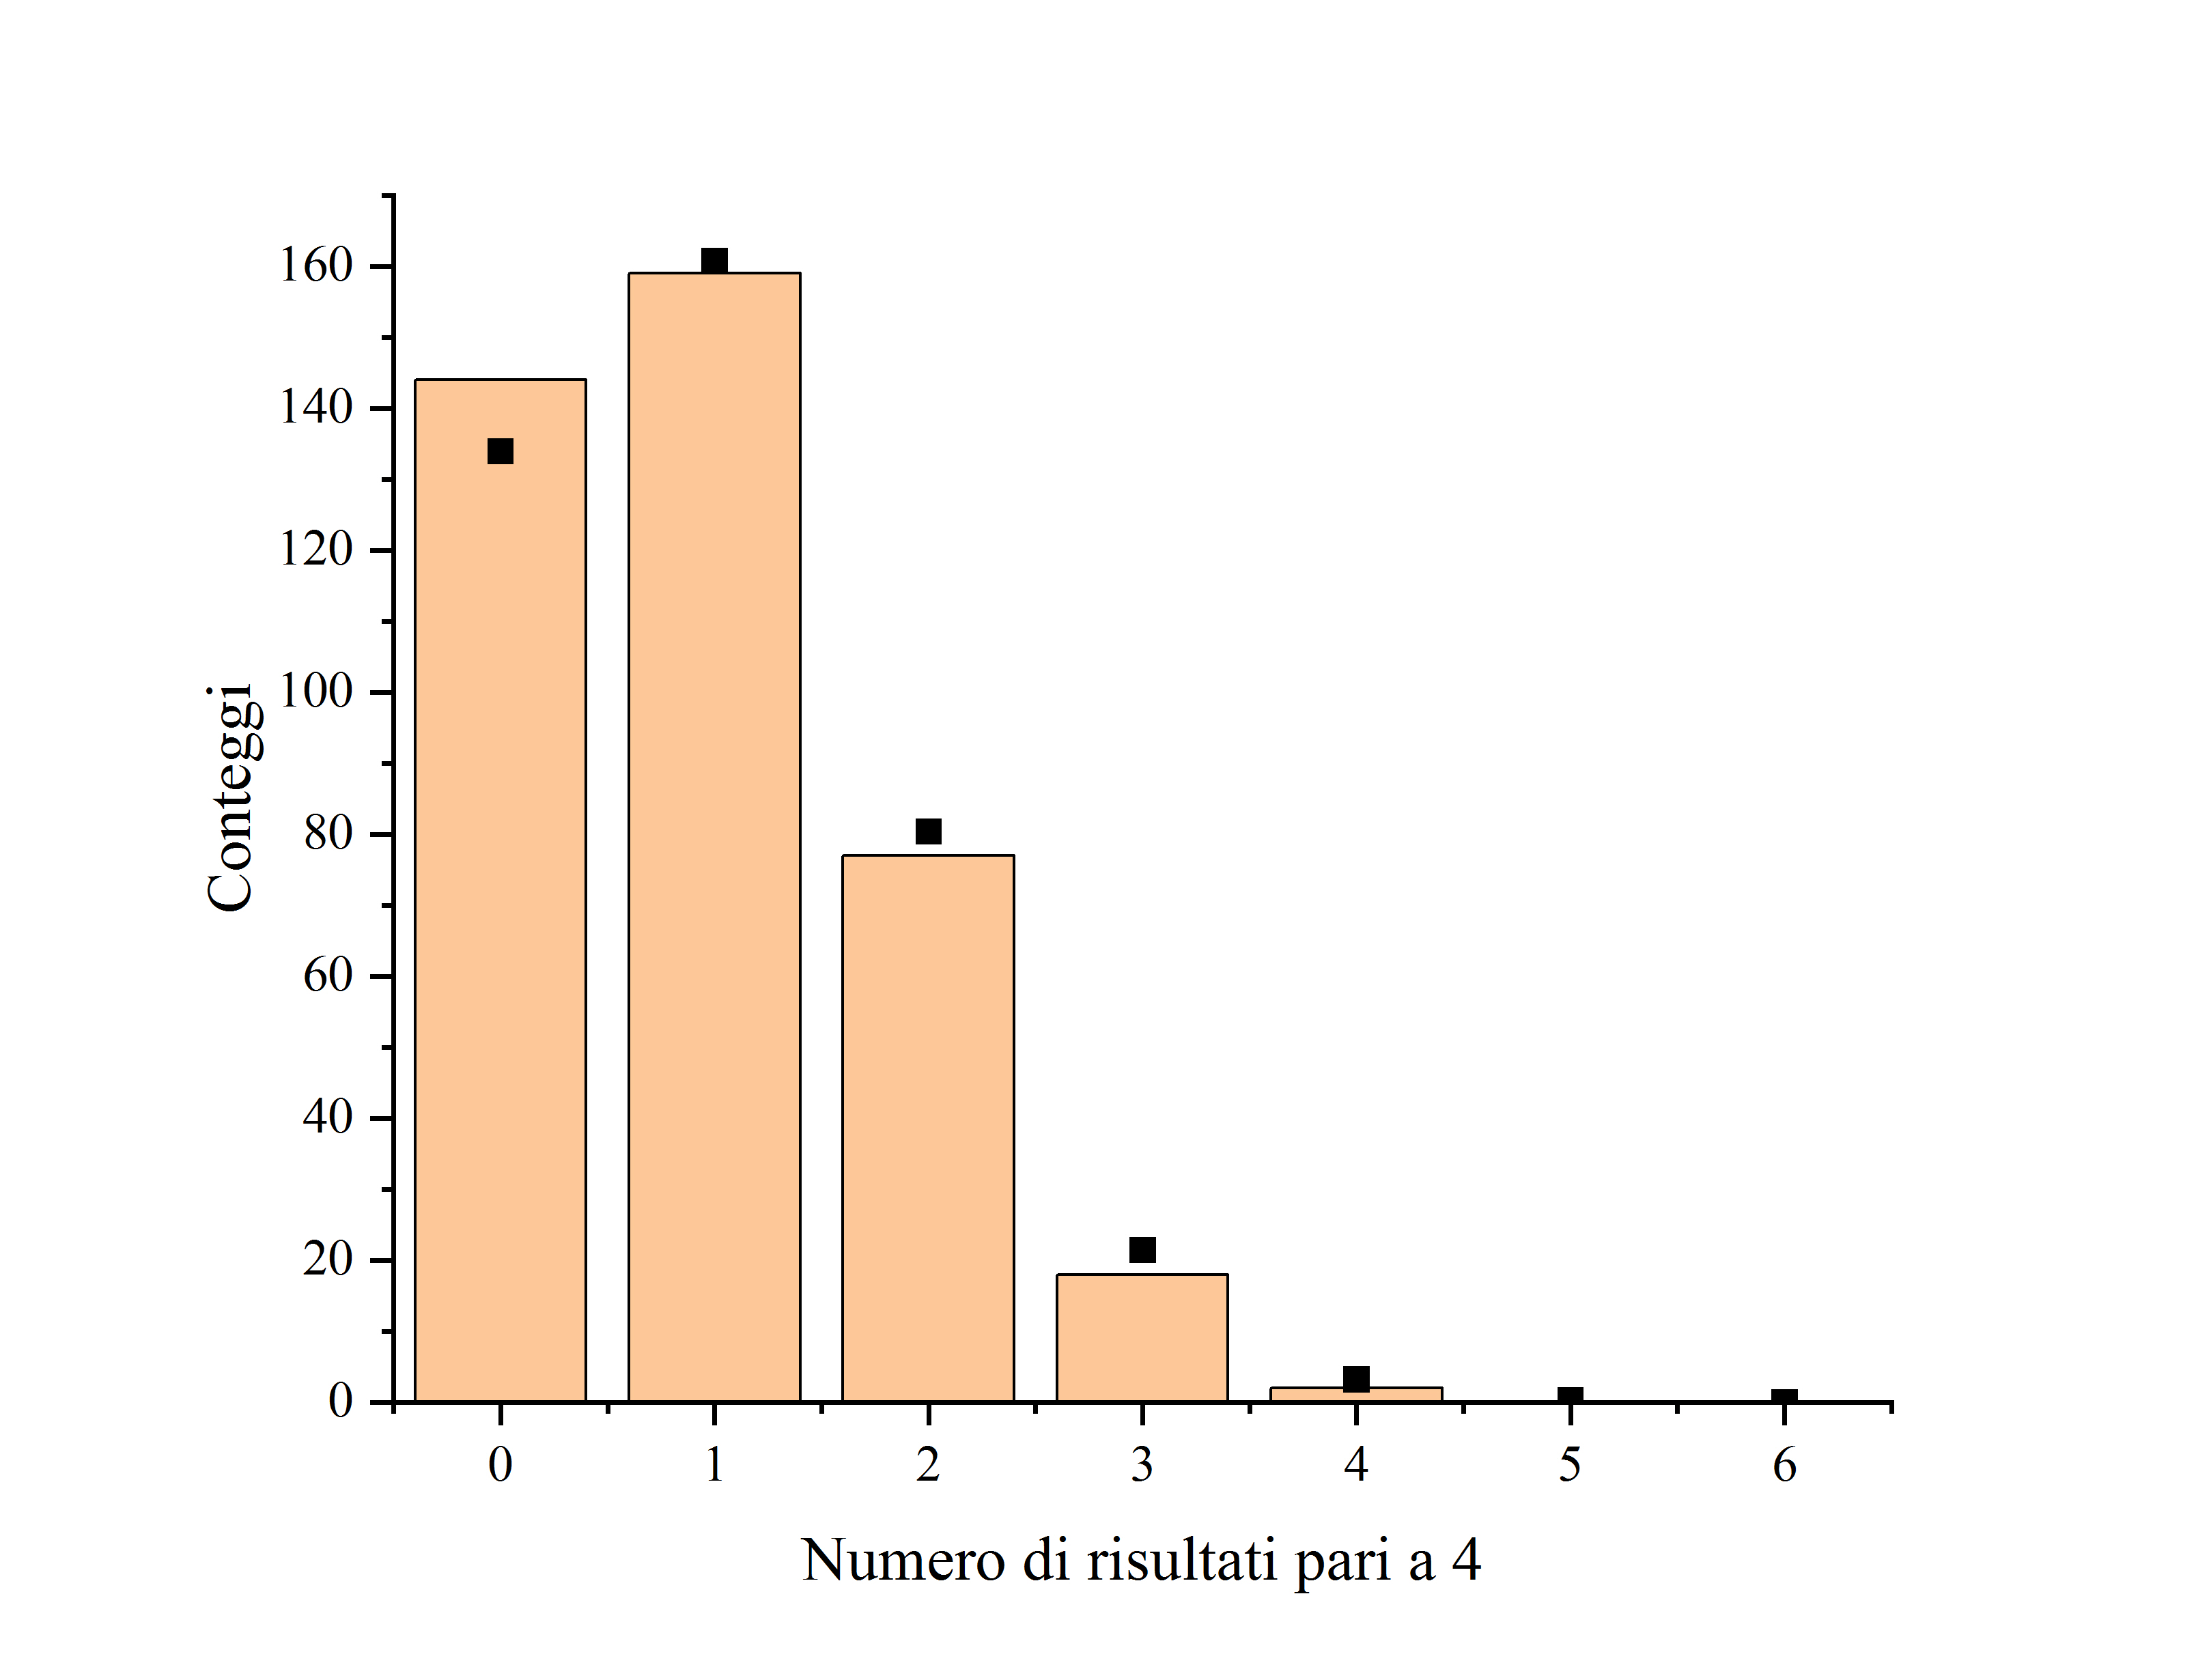
\includegraphics[trim={2cm .5cm 2.4cm 2.1cm},clip,width=.5\textwidth]{img/Dadi4.jpg}
        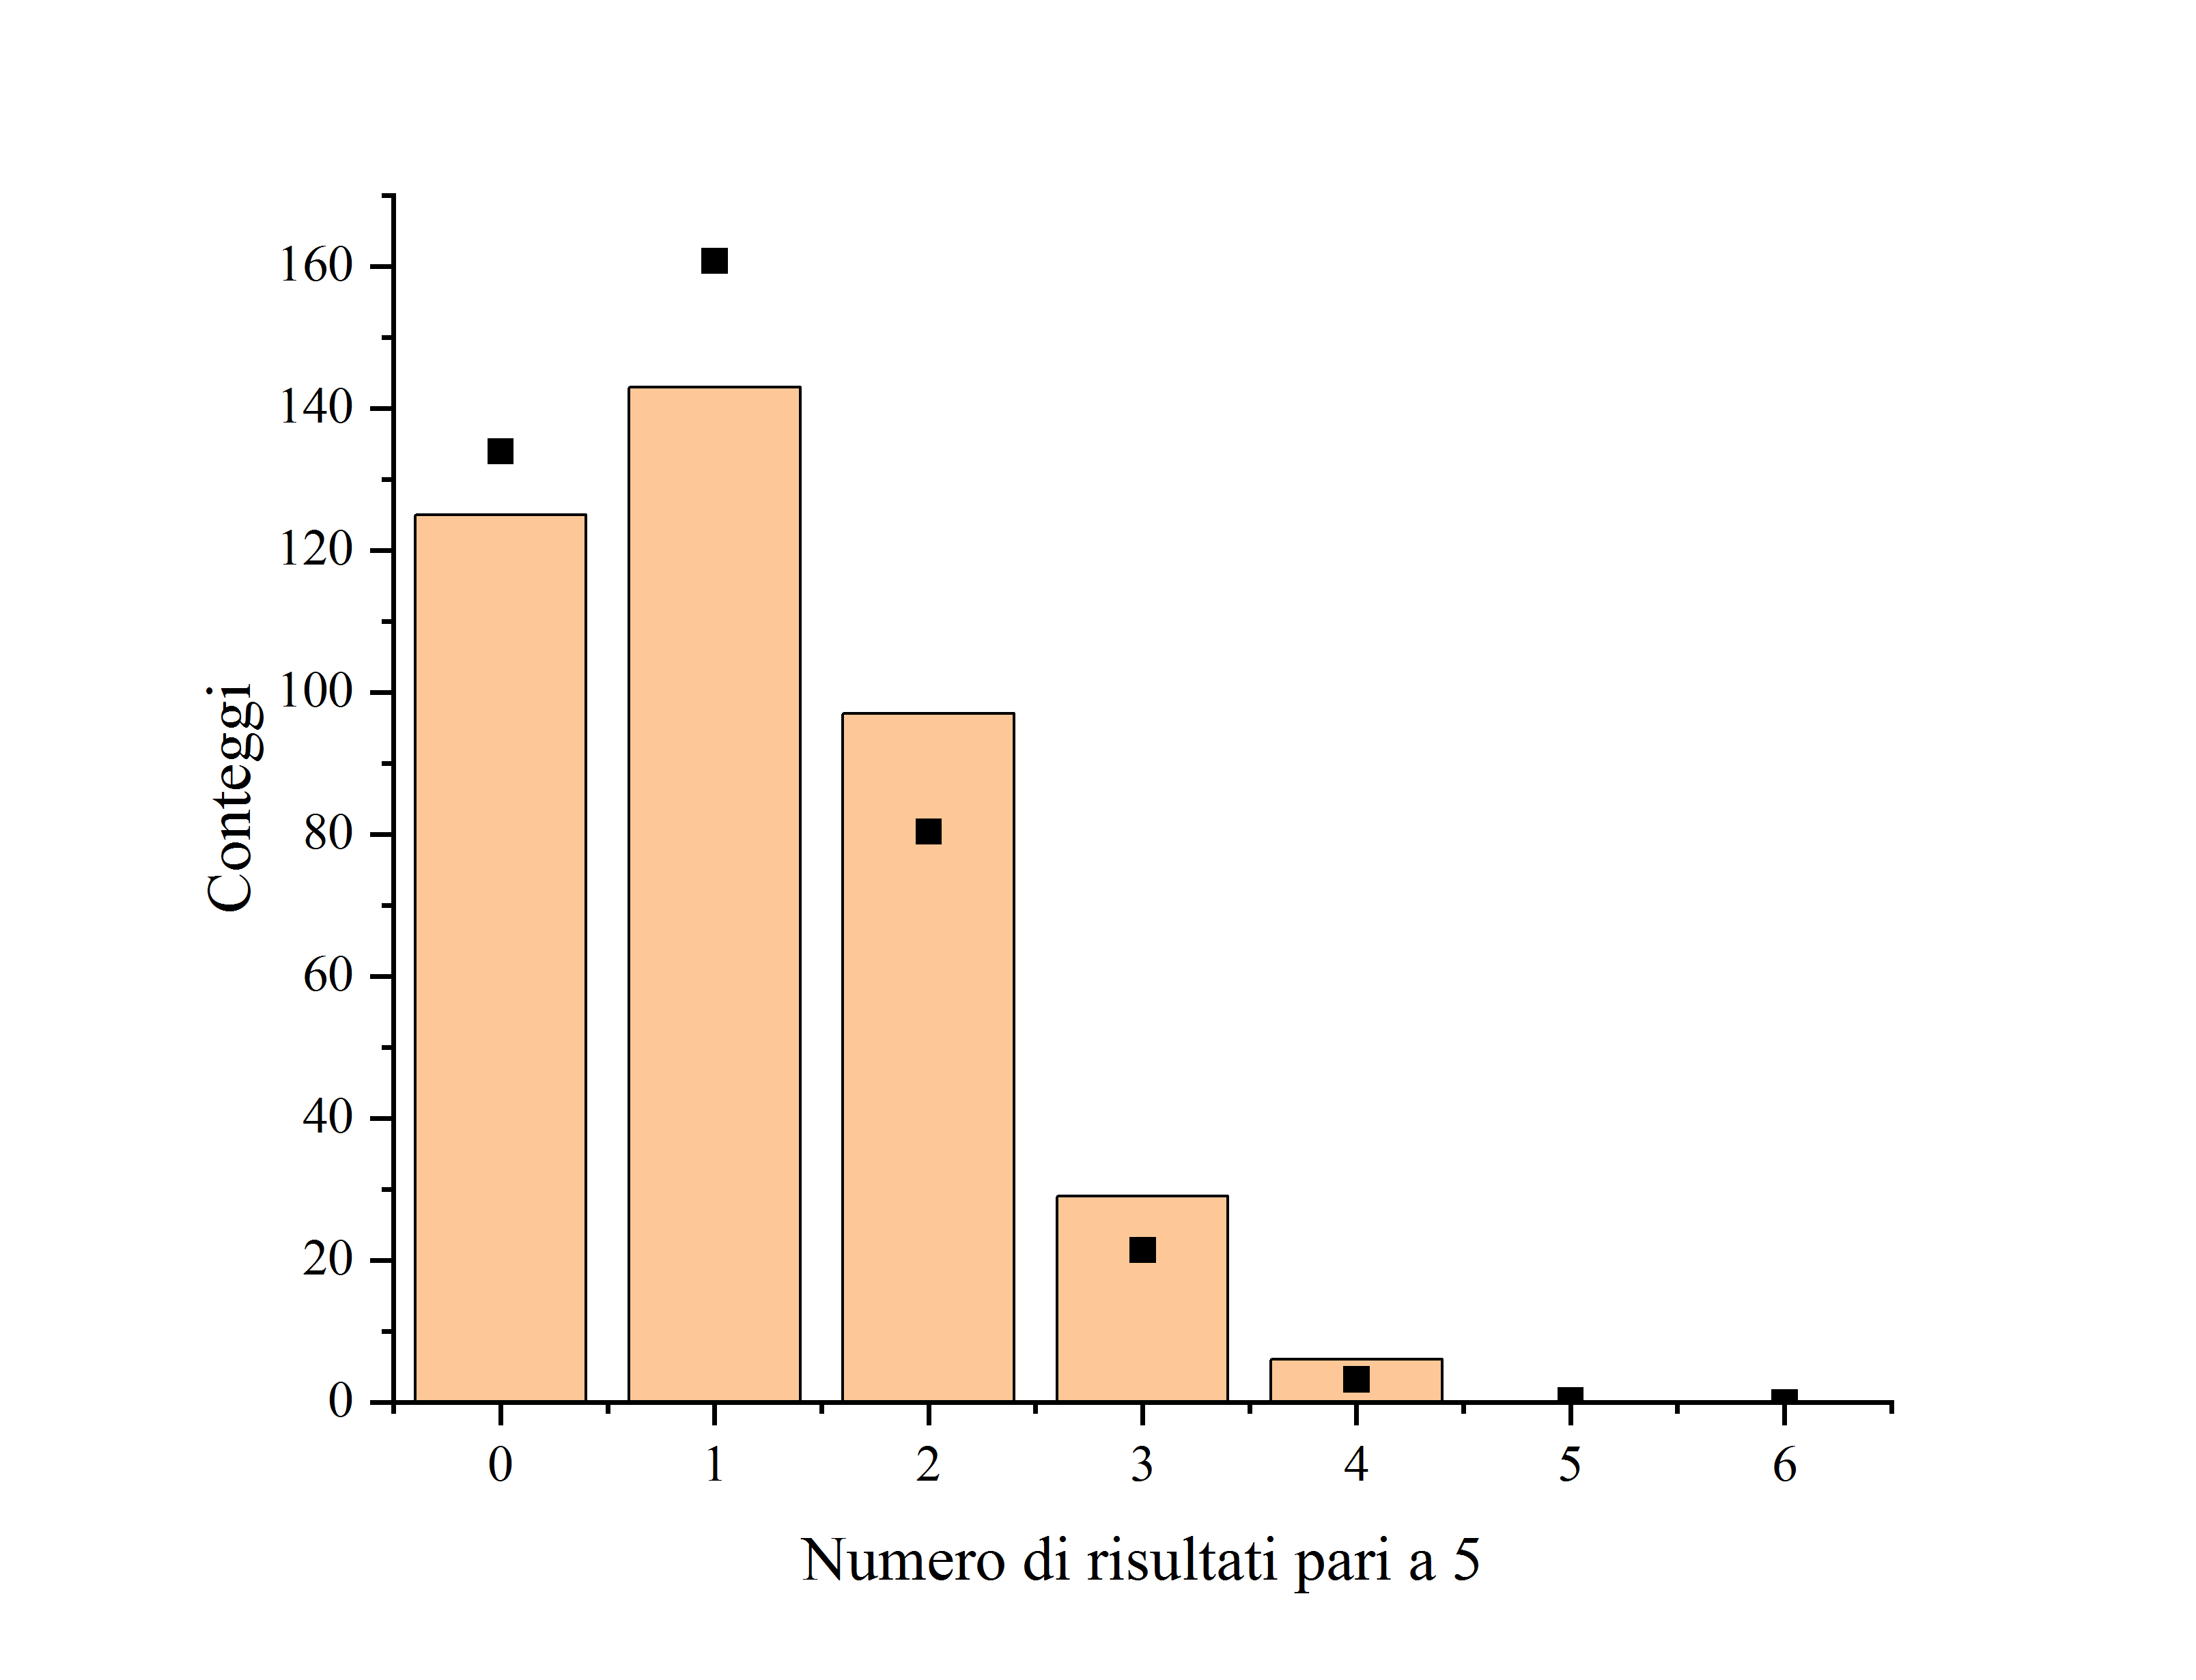
\includegraphics[trim={2cm .5cm 2.4cm 2.1cm},clip,width=.5\textwidth]{img/Dadi5.jpg}
        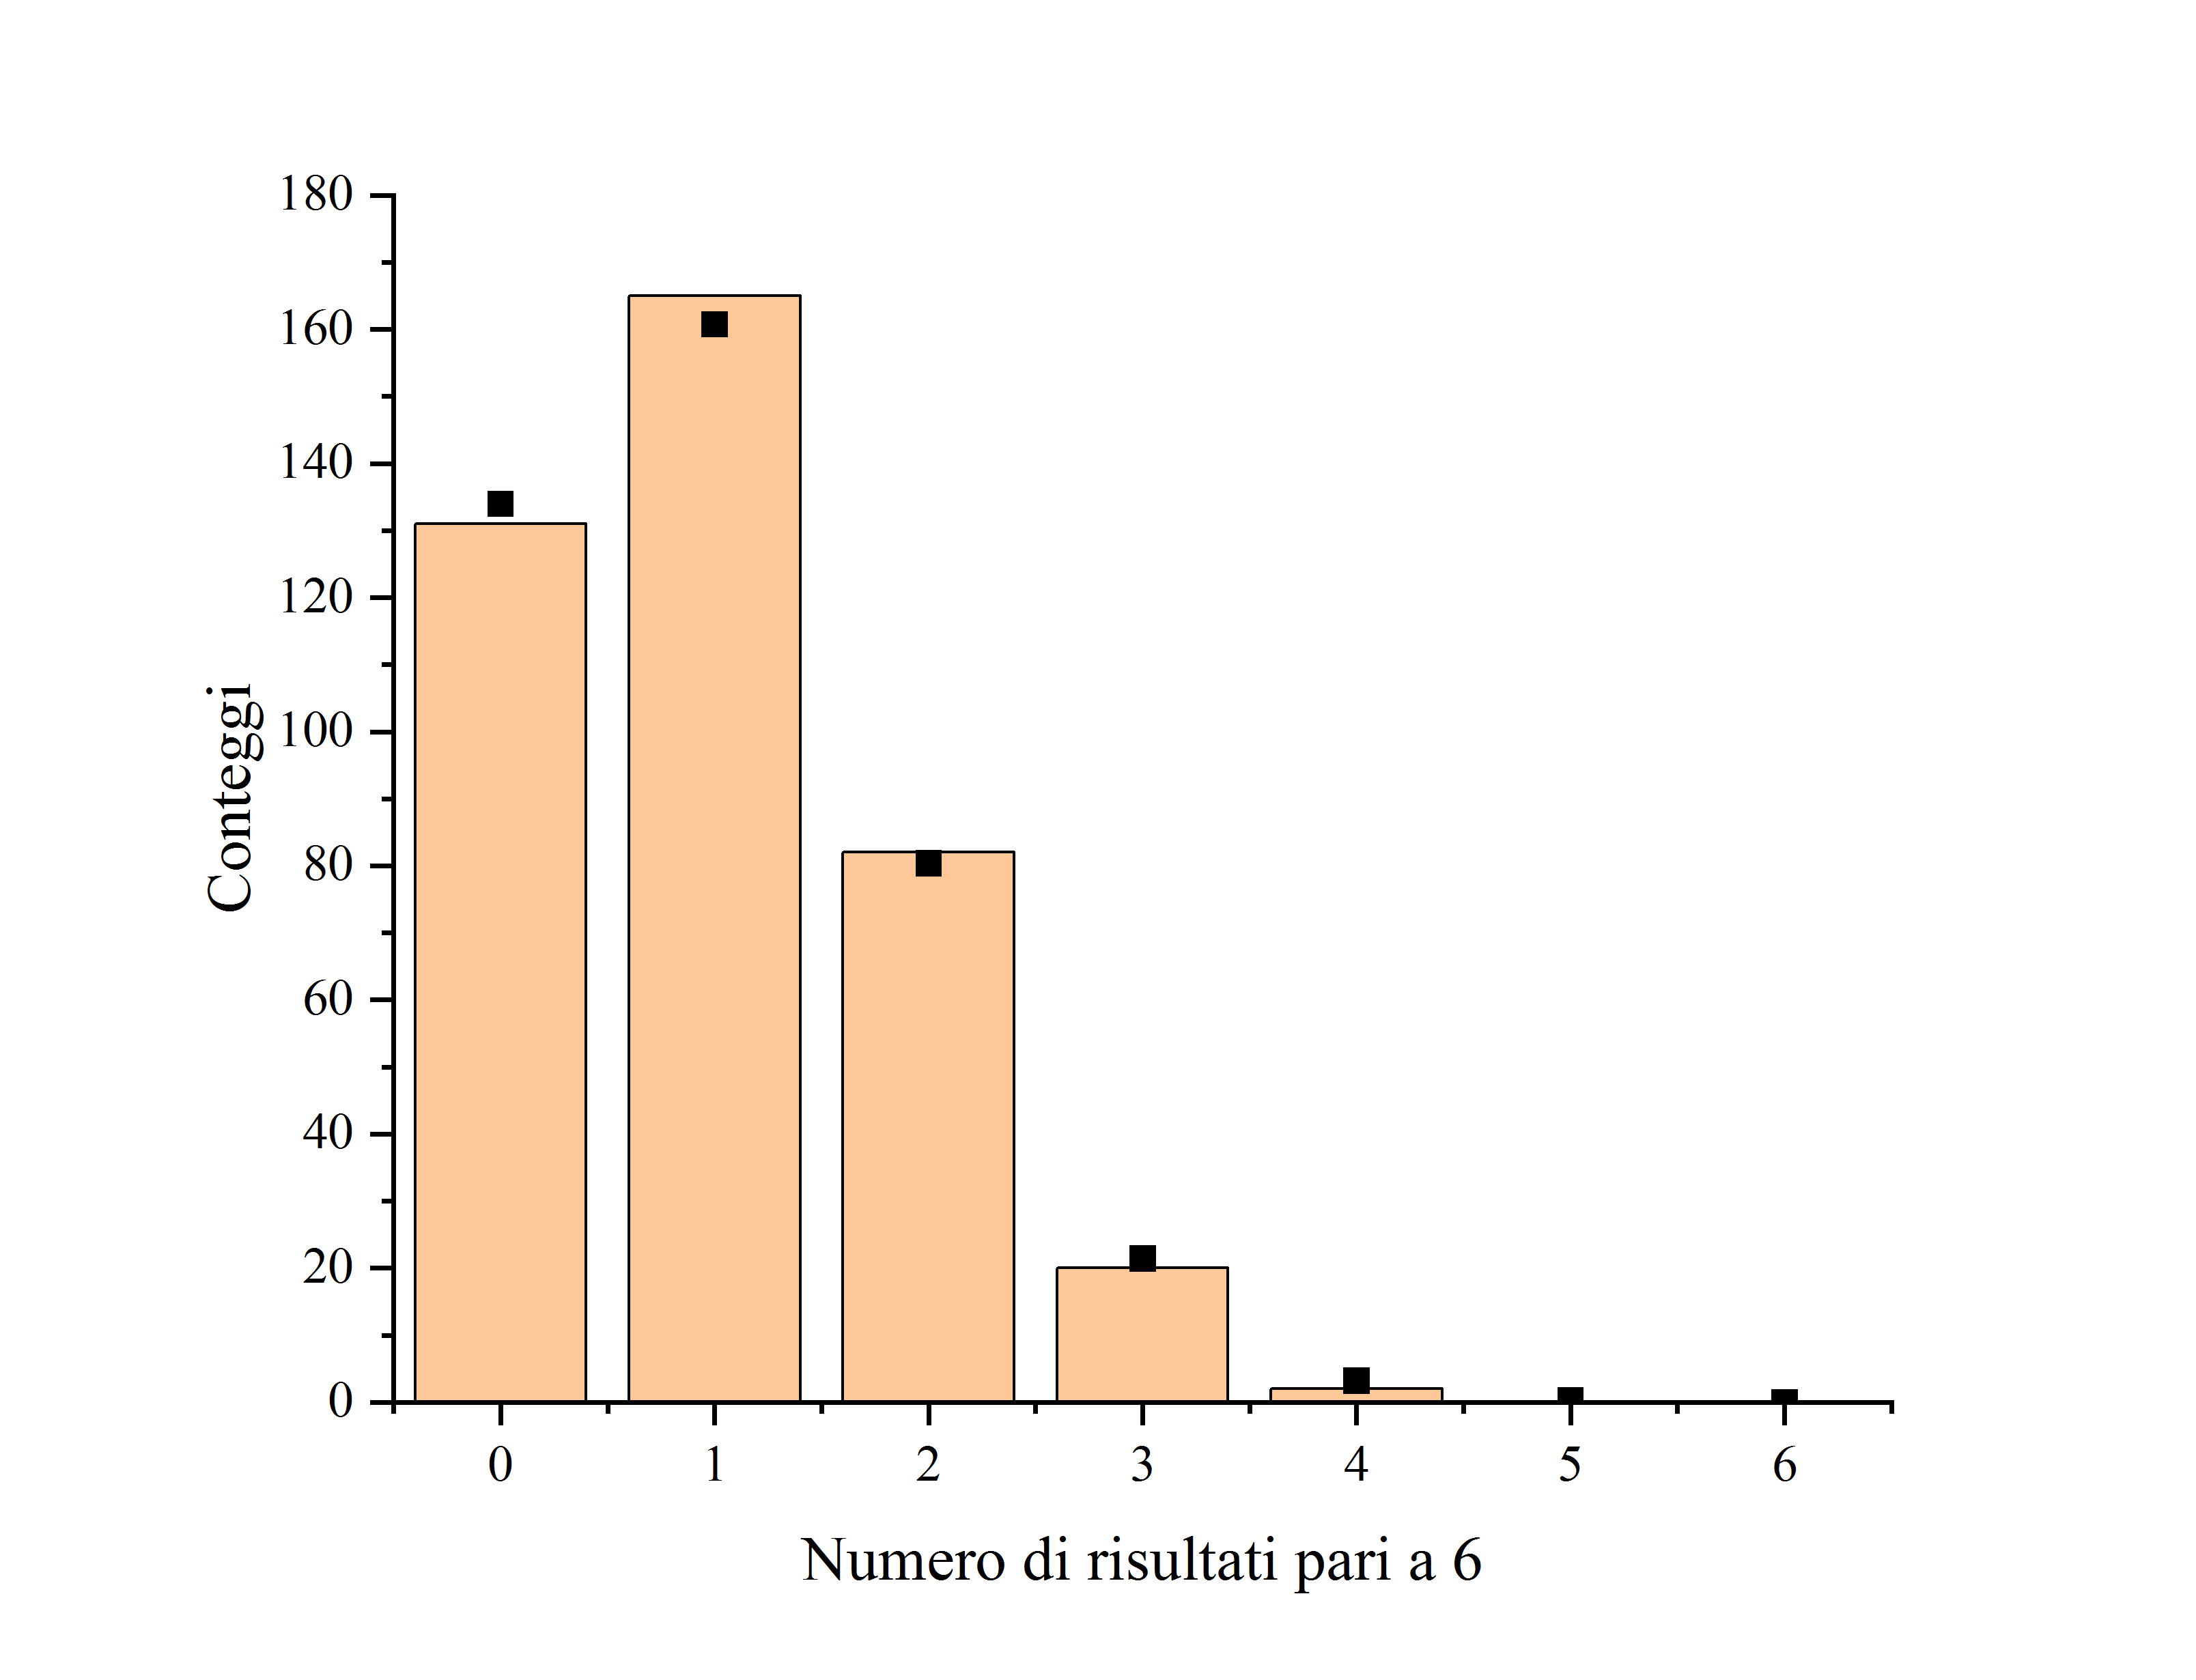
\includegraphics[trim={2cm .5cm 2.4cm 2.1cm},clip,width=.5\textwidth]{img/Dadi6.jpg}
    \end{figure}
\end{center}

Come è possibile osservare da questi grafici, i risultati riportati sembrano seguire
grossomodo la distribuzione teorica. Tuttavia, presentano deviazioni osservabili; il
gruppo di lavoro ritiene che ciò sia principalmente dovuto al ridotto numero di lanci.

% \subsubsection*{Onestà dei dadi}
% Avendo segnato tutti i risultati di ogni dado, possiamo inoltre stimare se i dadi che
% abbiamo utilizzato sono truccati o meno. Infatti, su un dado onesto ci aspettiamo
% che escano tutti i risultati possibili con equa probabilità. Di seguito riportiamo
% gli istogrammi dei valori usciti su ogni dado.

% \begin{figure*}
%     \caption{...}
% \end{figure*}

\subsection{Simulazione}
Tramite un programma da noi scritto e compilato\footnote{\emph{Vedi} Appendice A},
simuliamo la stessa esperienza con $10^{12}$ lanci dei sei dadi, al fine di
verificare la legge dei grandi numeri.

Di seguito riportiamo, in un istogramma, i risultati della simulazione.

\begin{center}
    \begin{figure}[H]
        % trim={< v > ^}
        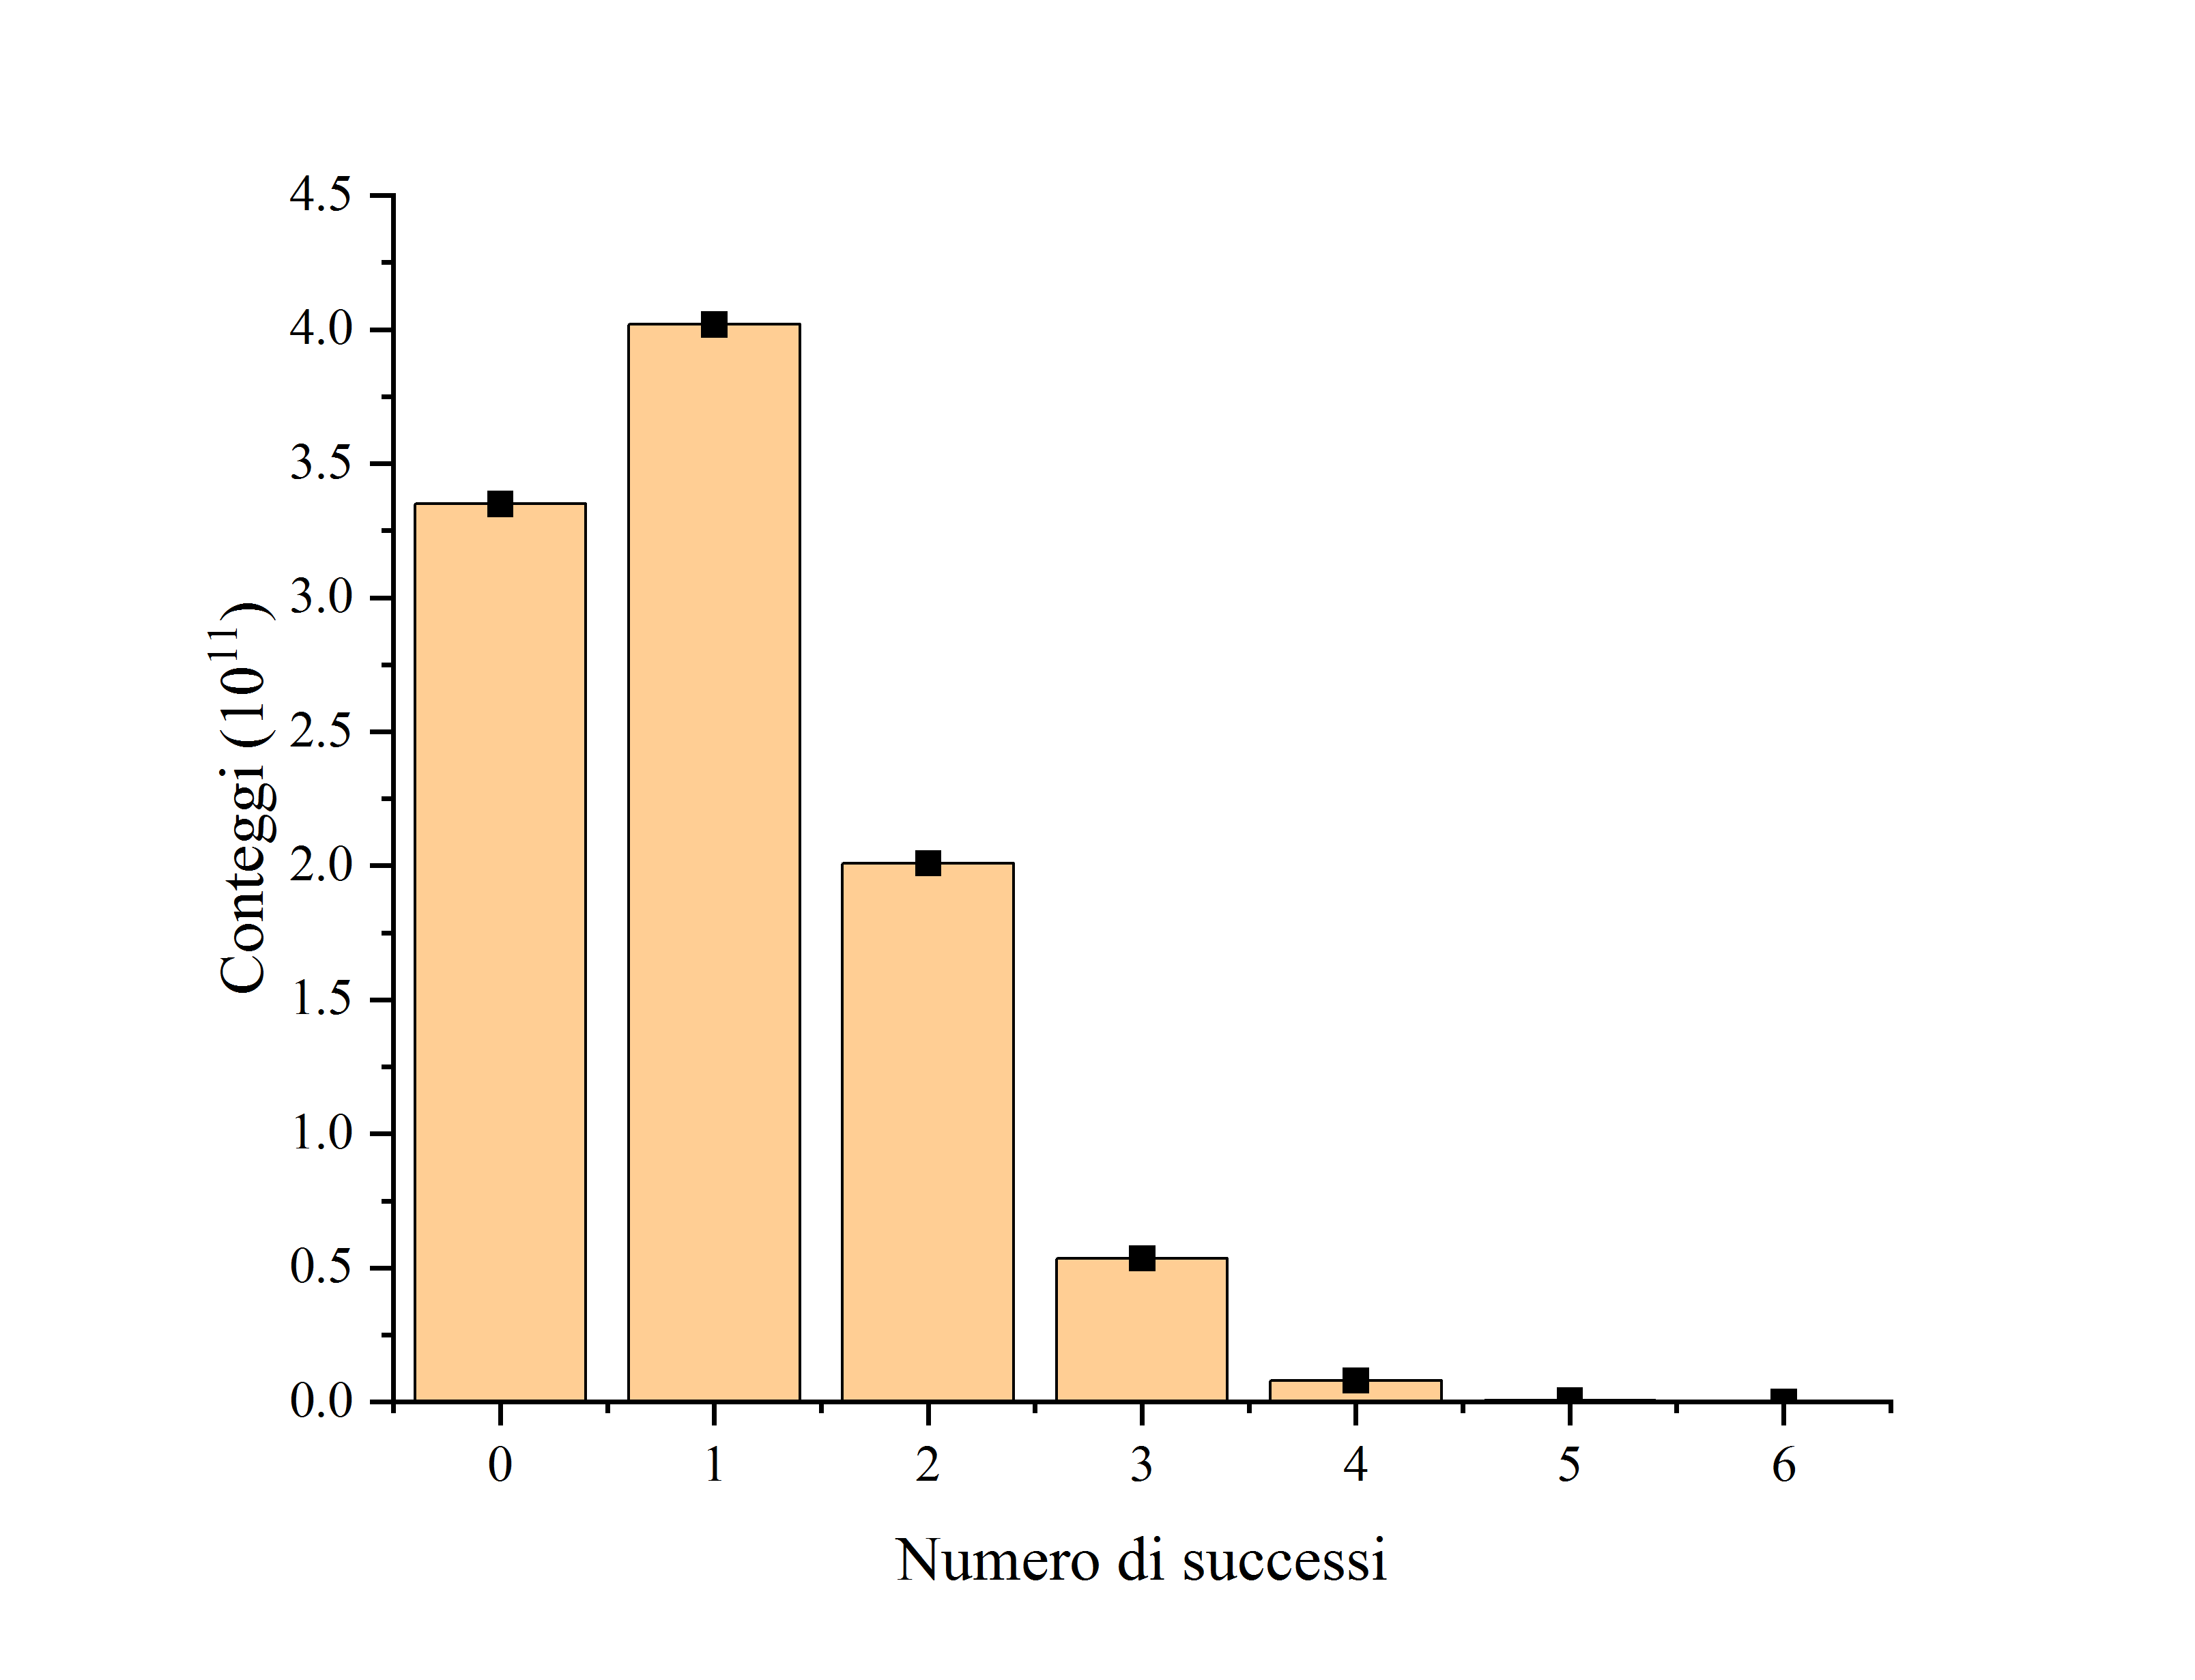
\includegraphics[trim={2cm .5cm 2cm 2.1cm},clip,width=\textwidth]{img/DadiSimul.png}
    \end{figure}
\end{center}

Come è possibile osservare dal grafico, i risultati della simulazione sono, in proporzione,
talmente vicini alla distribuzione teorica da risultare pressoché indistinguibili da essa.

Ciò è in accordo con la legge dei grandi numeri, secondo la quale, al crescere del
numero di prove, la distribuzione di probabilità rappresenta sempre meglio i
risultati ottenuti, normalizzati.

\pagebreak
\section{Processo di Poisson}
\subsection{Materiali e strumenti di misura utilizzati}
\begin{center}
    \begin{tblr}{ |Q[l,m]|Q[c,m]|Q[c,m]|Q[c,m]| }
        \hline
        \textbf{Strumento di misura} & \textbf{\:\:\:\:\:Soglia\:\:\:\:\:} & \textbf{Portata} & \textbf{Sensibilità} \\
        \hline
        {Contatore Geiger} & \qty{1}{conteggi \per s} & N./A. & \qty{1}{conteggi \per s} \\
        \hline[dashed]
        Metro a nastro & \qty{0.1}{cm} & \qty{300.0}{cm} & \qty{0.1}{cm} \\
        \hline
        \hline
        \textbf{Altro} & \SetCell[c=3]{l} \textbf{Descrizione/Note} \\
        \hline
        {Campione di $\Th$} & \SetCell[c=3]{l} {
            Componente di una lampada da campeggio
        } \\
        \hline
    \end{tblr}
\end{center}


\subsection{Esperienza e procedimento di misura}

Posizionato il contatore Geiger a una certa distanza $d_i$ dal campione di $\Th$
(con $i\in\left[1;4\right]\cap\mathbb{N}$),
definiamo una variabile aleatoria $x_i$ come il numero di raggi $\gamma$
emessi dal $\Th$ nell'arco di un secondo, nella direzione del contatore.
Allora, detta $\overline{x_i}$ la media teorica
% \footnote{
    % Che il parametro della distribuzione coincida con la media è facilmente
    % dimostrabile. Detto $\lambda$ quel parametro, vale:
    % \[\begin{aligned}
        % \overline{x_\gamma} &= \sum_{k=0}^{+\infty} k\,p(x_\gamma=k) =
        % \sum_{k=0}^{+\infty} k \frac{\lambda^k  e^{-\lambda}}{k!} =
        % e^{-\lambda} \sum_{k=0}^{+\infty} k \frac{\lambda^k}{k!} =
        % e^{-\lambda} \left(0 + \sum_{k=1}^{+\infty} k \frac{\lambda^k}{k!}\right) \\ &=
        % \lambda e^{-\lambda} \sum_{k=1}^{+\infty} \frac{\lambda^{k-1}}{(k-1)!} =
        % \lambda e^{-\lambda} \sum_{j=0}^{+\infty} \frac{\lambda^j}{j!} =
        % \lambda e^{-\lambda} e^\lambda =
        % \lambda\quad\square
    % \end{aligned}\]
% }
di $x_i$, la distribuzione di probabilità di $x_i$ è data da una Poissoniana:
\[
    p(x_i=k)=\frac{\overline{x_i}^k e^{-\overline{x_i}}}{k!}
    \qquad
    \forall k\in\mathbb{N}
\]
Il valore di $\overline{x_i}$ è legato alla distanza $d_i$, al raggio $r$
della finestra del contatore, al tempo di dimezzamento $T_\frac{1}{2}$ del
$\Th$ e al numero $N$ di atomi di $\Th$ secondo la seguente relazione\footnote{
    Il numero medio $\overline{X}$ di raggi $\gamma$ emessi dal campione è:
    \[
        \overline{X} = \frac{N}{\tau} = \frac{N\ln{2}}{T_\frac{1}{2}}
    \]
    con $\tau=\frac{1}{\ln{2}}T_\frac{1}{2}$ il tempo caratteristico del $\Th$.
    Tuttavia, poiché la superficie di acquisizione è $\pi r^2$, e non $4\pi d_i^2$,
    dobbiamo moltiplicare per il rapporto fra le aree:
    \[
        \overline{x_i} = \frac{\pi r^2}{4\pi d_i^2} \overline{X} =
        \frac{Nr^2\ln{2}}{4 d_i^2 T_\frac{1}{2}}
    \]
    Infine, dobbiamo ricordare che il contatore Geiger non rileva soltanto le
    radiazioni emesse dal campione. Possiamo tenere conto di tutti gli altri
    contributi introducendo un termine costante $\overline{x_0}$, che chiameremo
    “media dei conteggi relativi alla radioattività ambientale”.
    Si ottiene così la relazione riportata.
}:
\[
    \overline{x_i} = \frac{Nr^2\ln{2}}{4 d_i^2 T_\frac{1}{2}} + \overline{x_0}
\]
D'ora in avanti indicheremo con $\xi$ la costante $\frac{r^2\ln{2}}{4T_\frac{1}{2}}$.
La relazione diventa allora:
\[\overline{x_i} = N\xi d_i^{-2} + \overline{x_0}\]

Per ogni distanza $d_i$, il gruppo di lavoro ha acquisito ripetutamente il valore di
$x_i$ per un tempo complessivo di circa un'ora\footnote{
    Abbiamo scelto deliberatamente di acquisire esattamente 3657 secondi in quanto
    $3657$ minimizza la funzione
    $f(x)=\left\{\frac{x}{\pi}\right\}=\frac{x}{\pi} - \left\lfloor\frac{x}{\pi}\right\rfloor$
    meglio di $3600$.
} ($\qty{3657}{s}$); ha poi acquisito nuovamente $x_4$ col contatore Geiger rivolto in
direzione opposta, per avere una stima diretta di $\overline{x_0}$.

Di seguito riportiamo gli istogrammi dei dati così raccolti,
assieme ai valori attesi, calcolati mediante la distribuzione teorica.

\begin{center}
    \begin{figure}[H]
        % trim={< v > ^}
        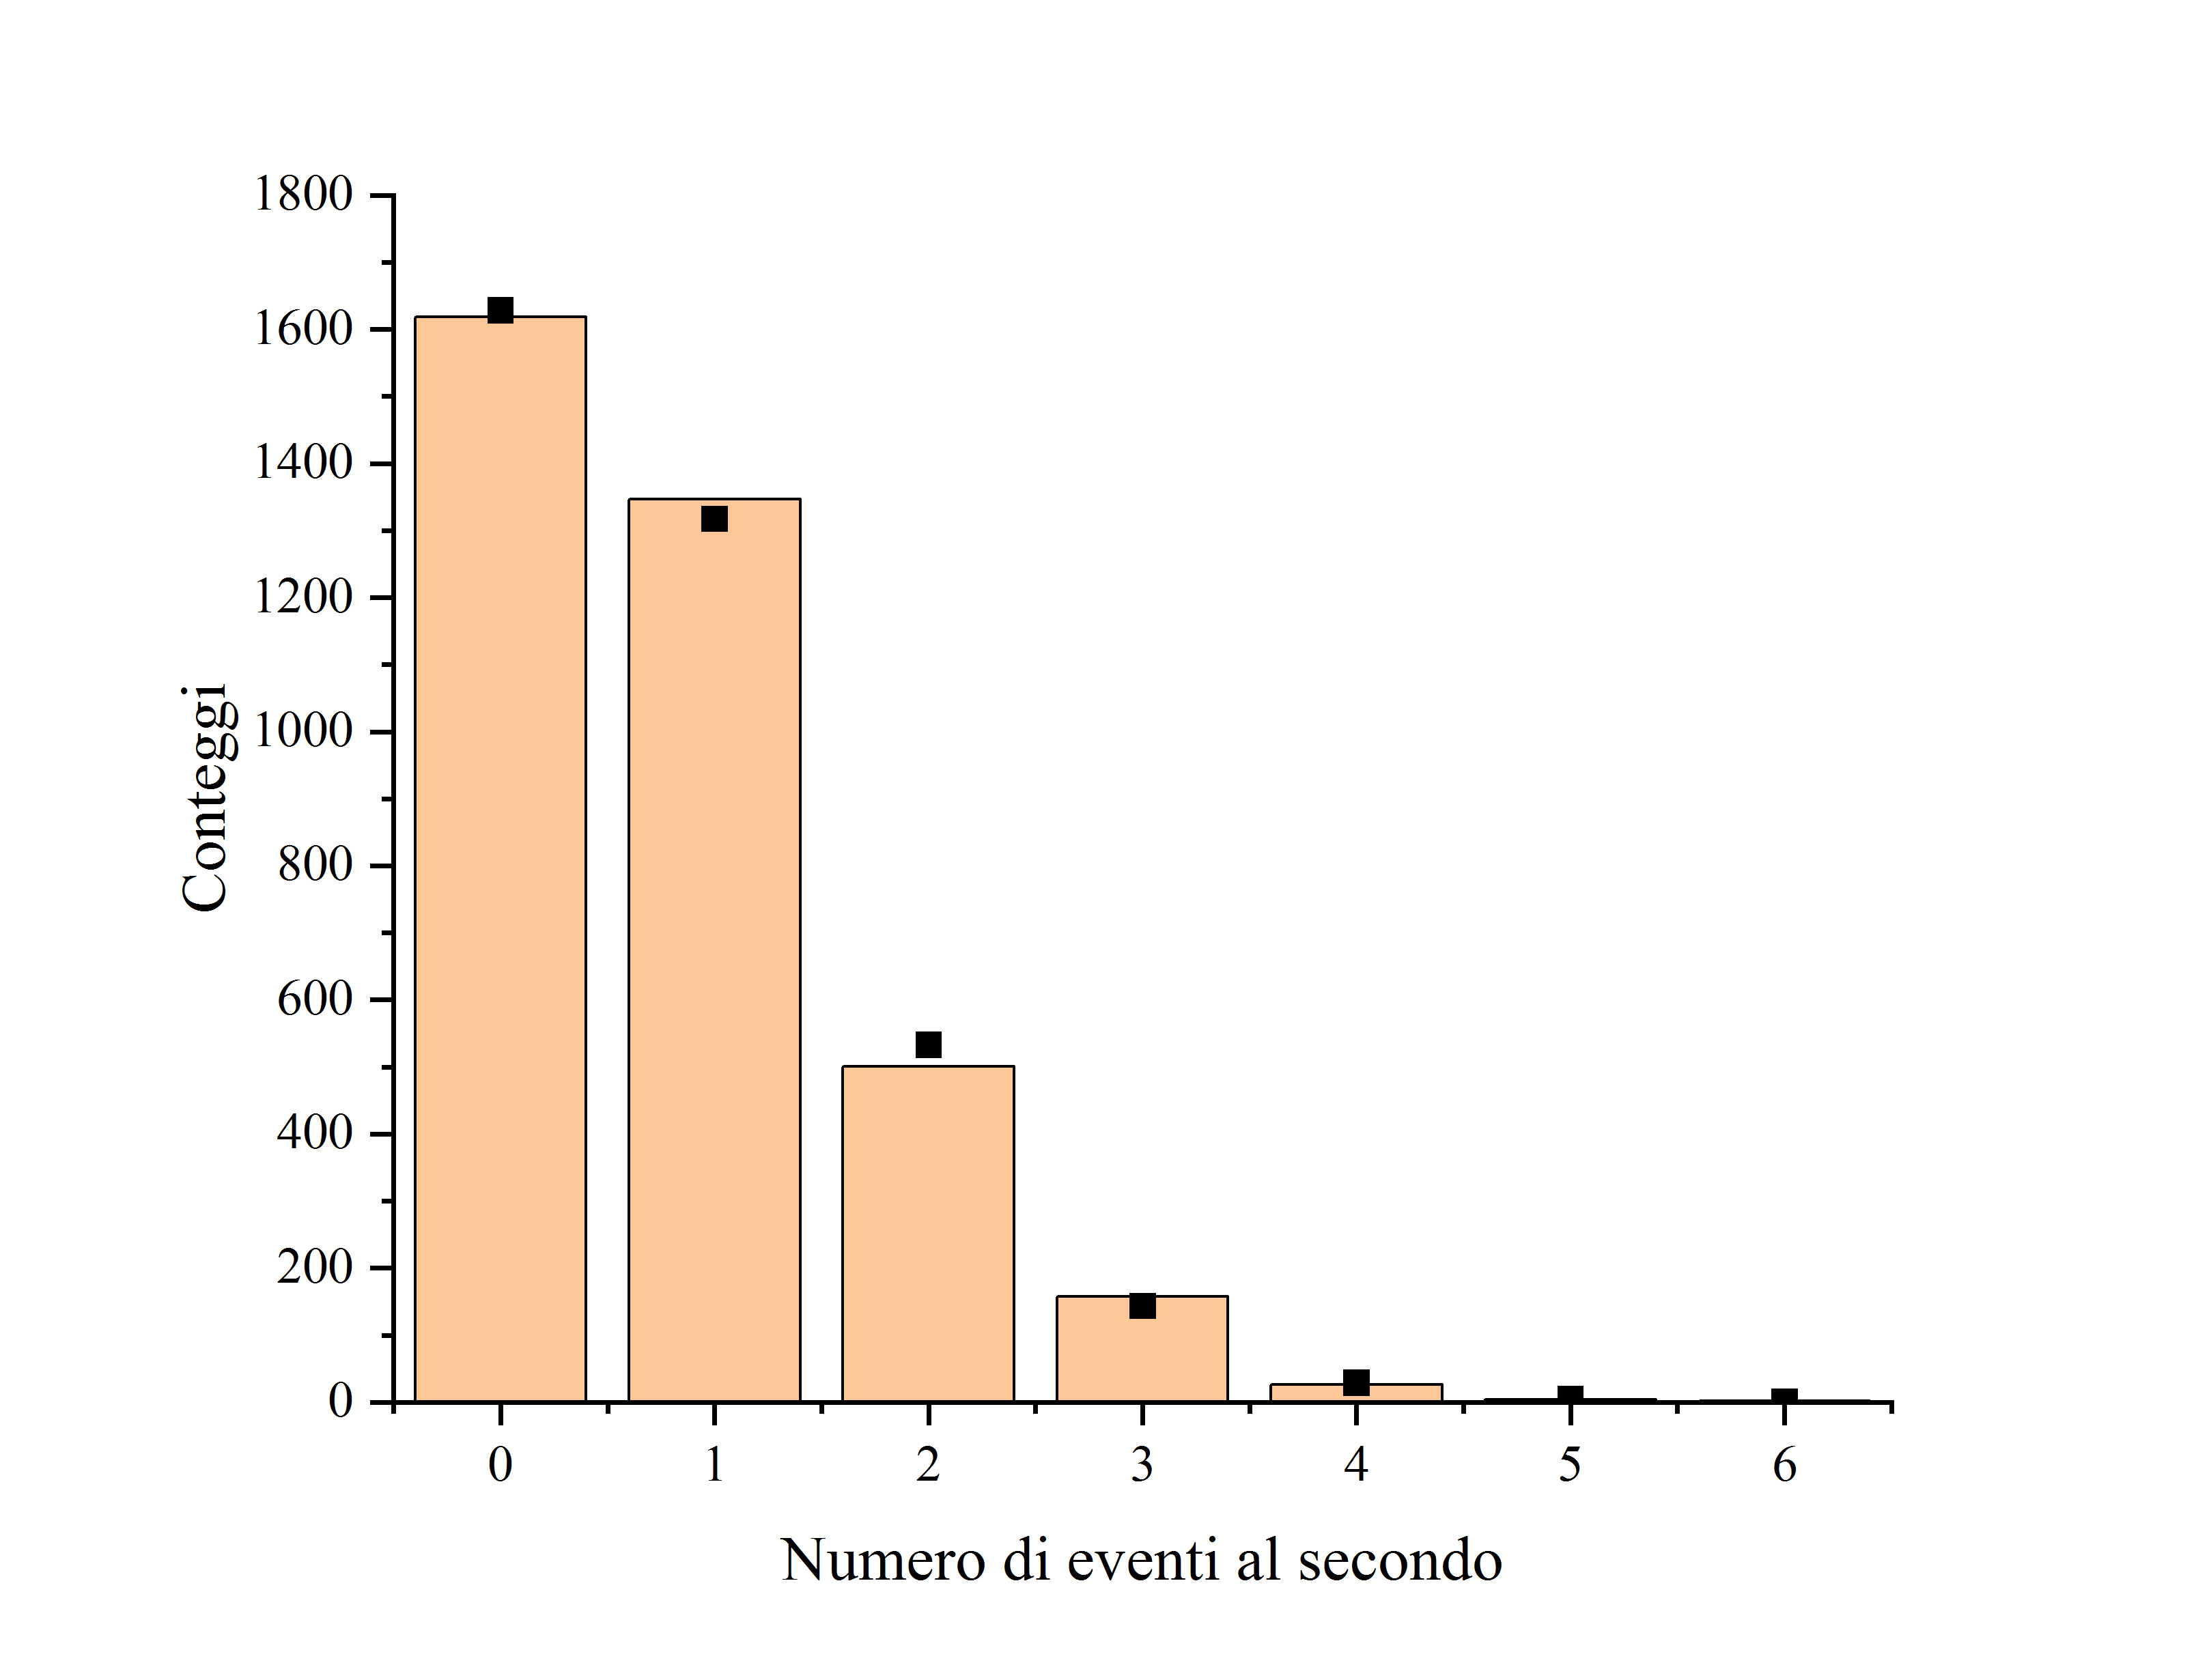
\includegraphics[trim={2cm .5cm 2.4cm 2.1cm},clip,width=.5\textwidth]{img/Geiger2.jpg}
        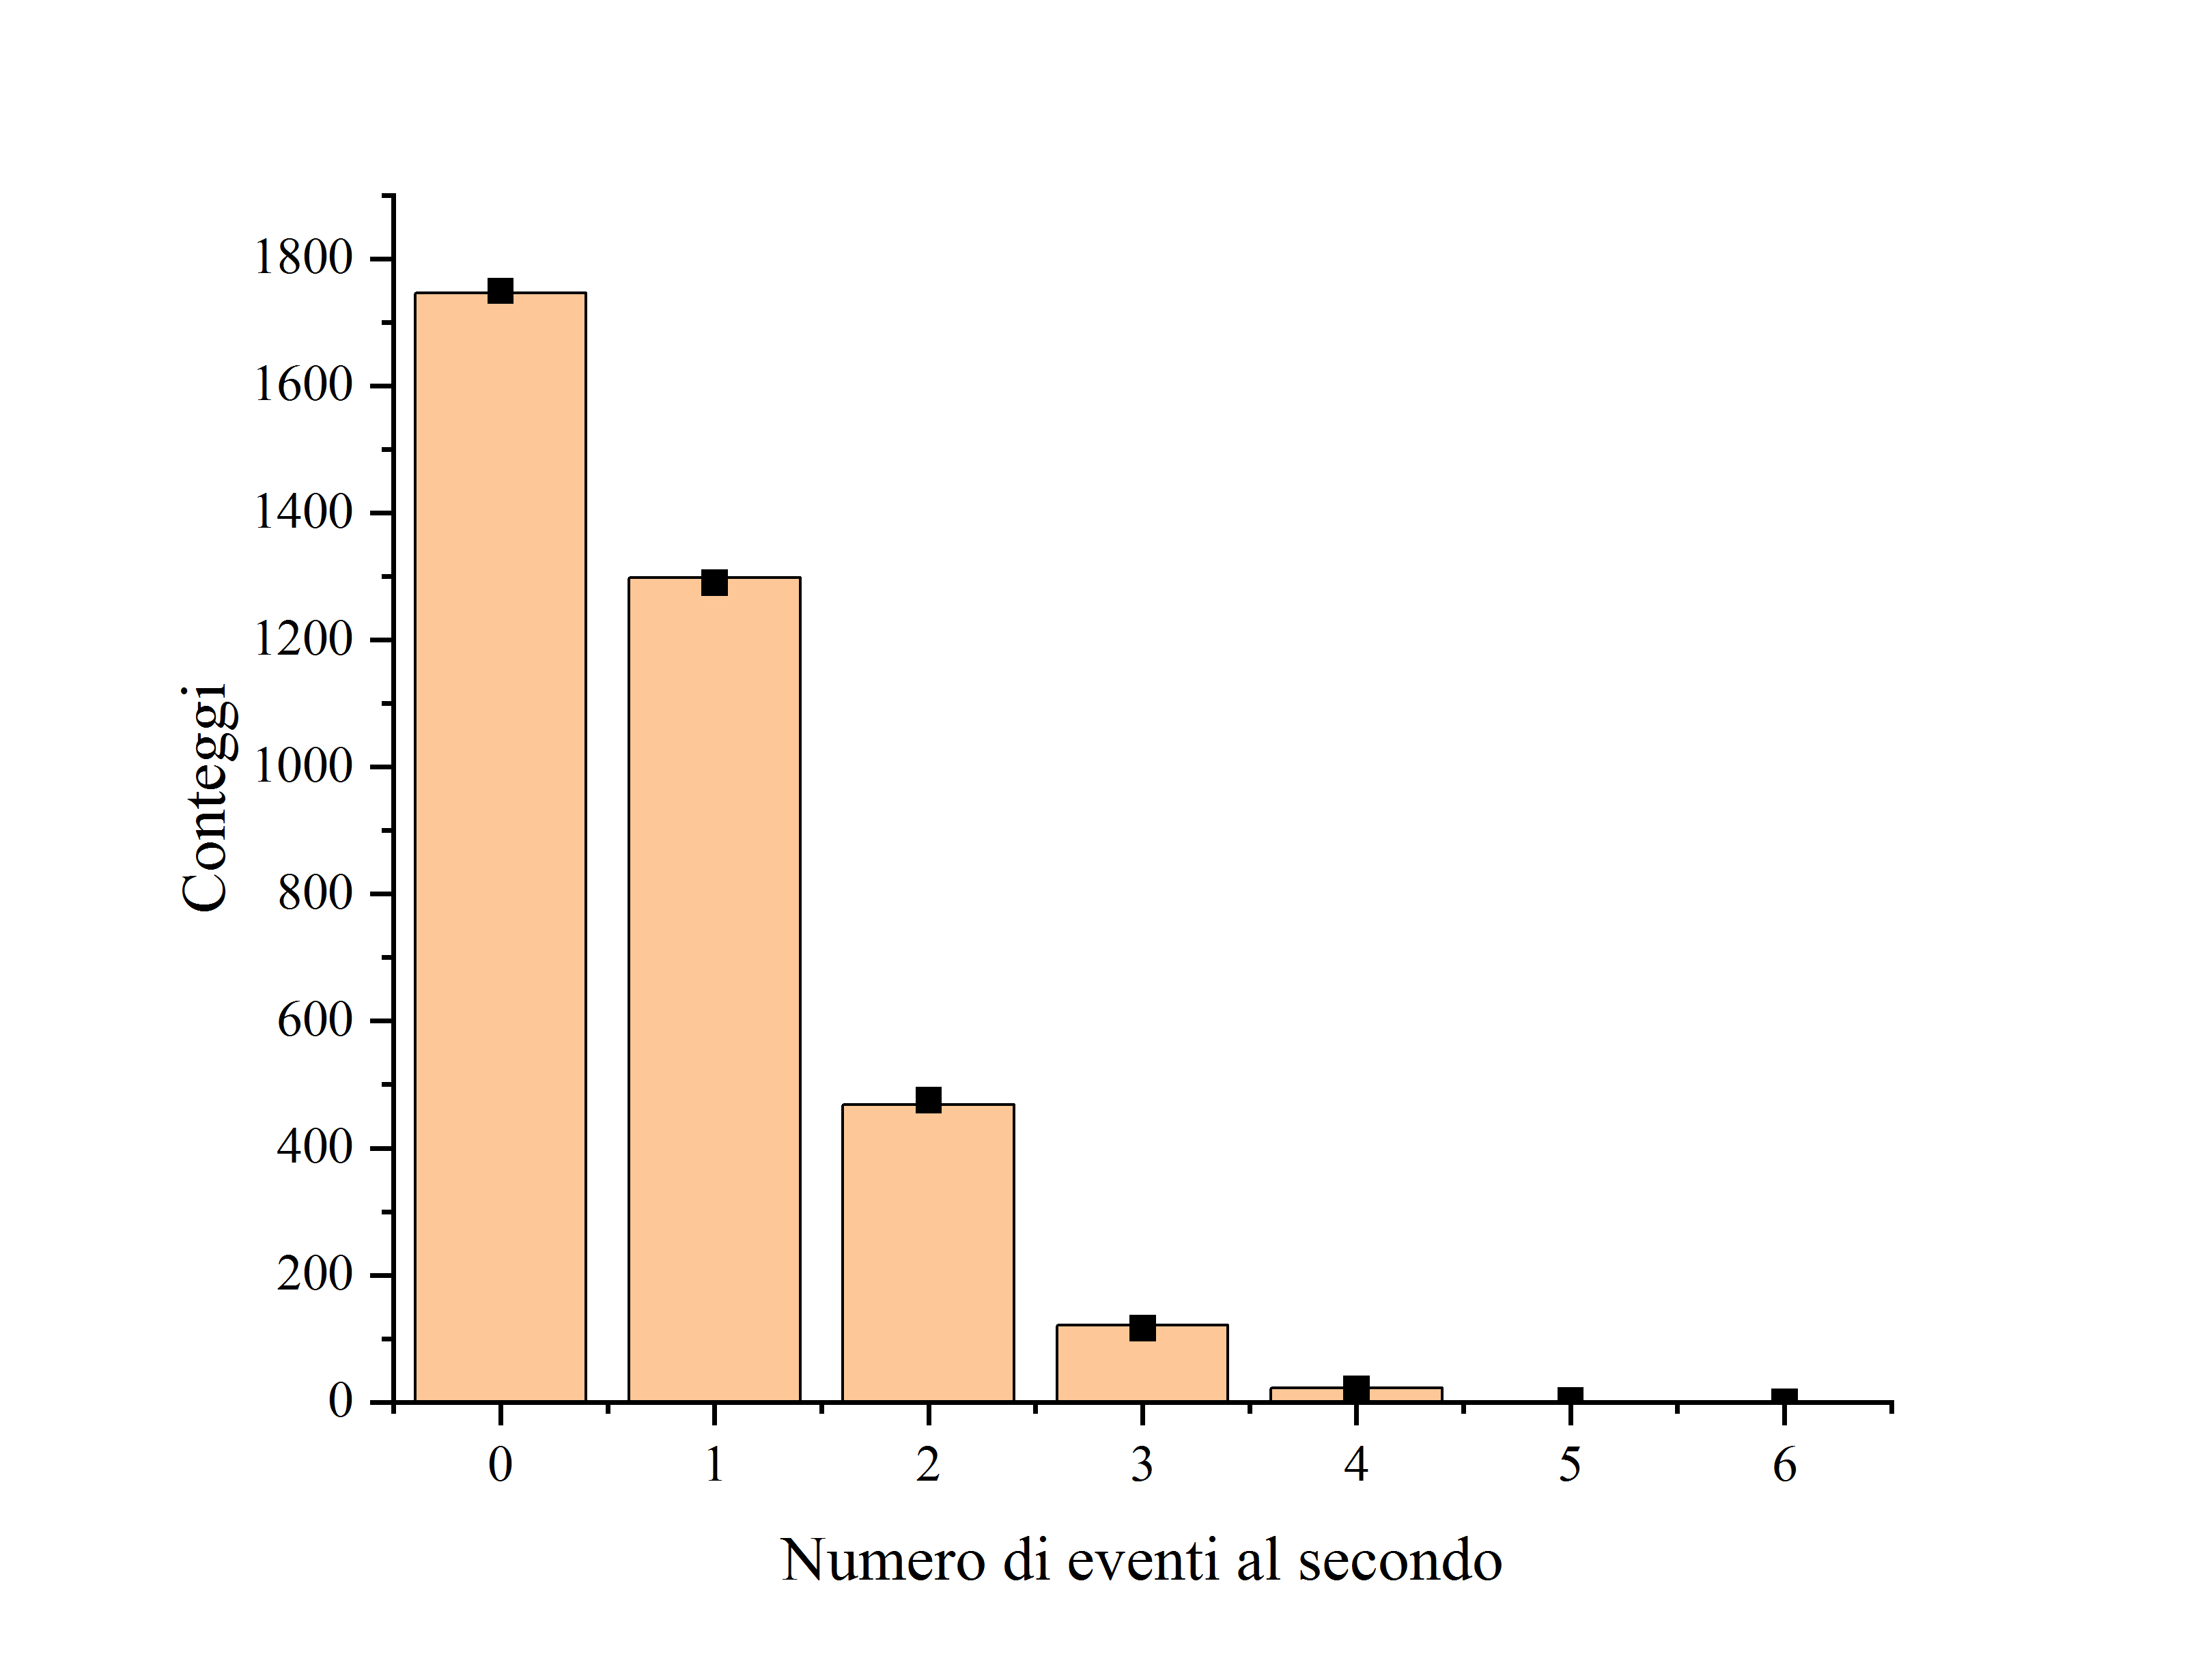
\includegraphics[trim={2cm .5cm 2.4cm 2.1cm},clip,width=.5\textwidth]{img/Geiger1.jpg}
        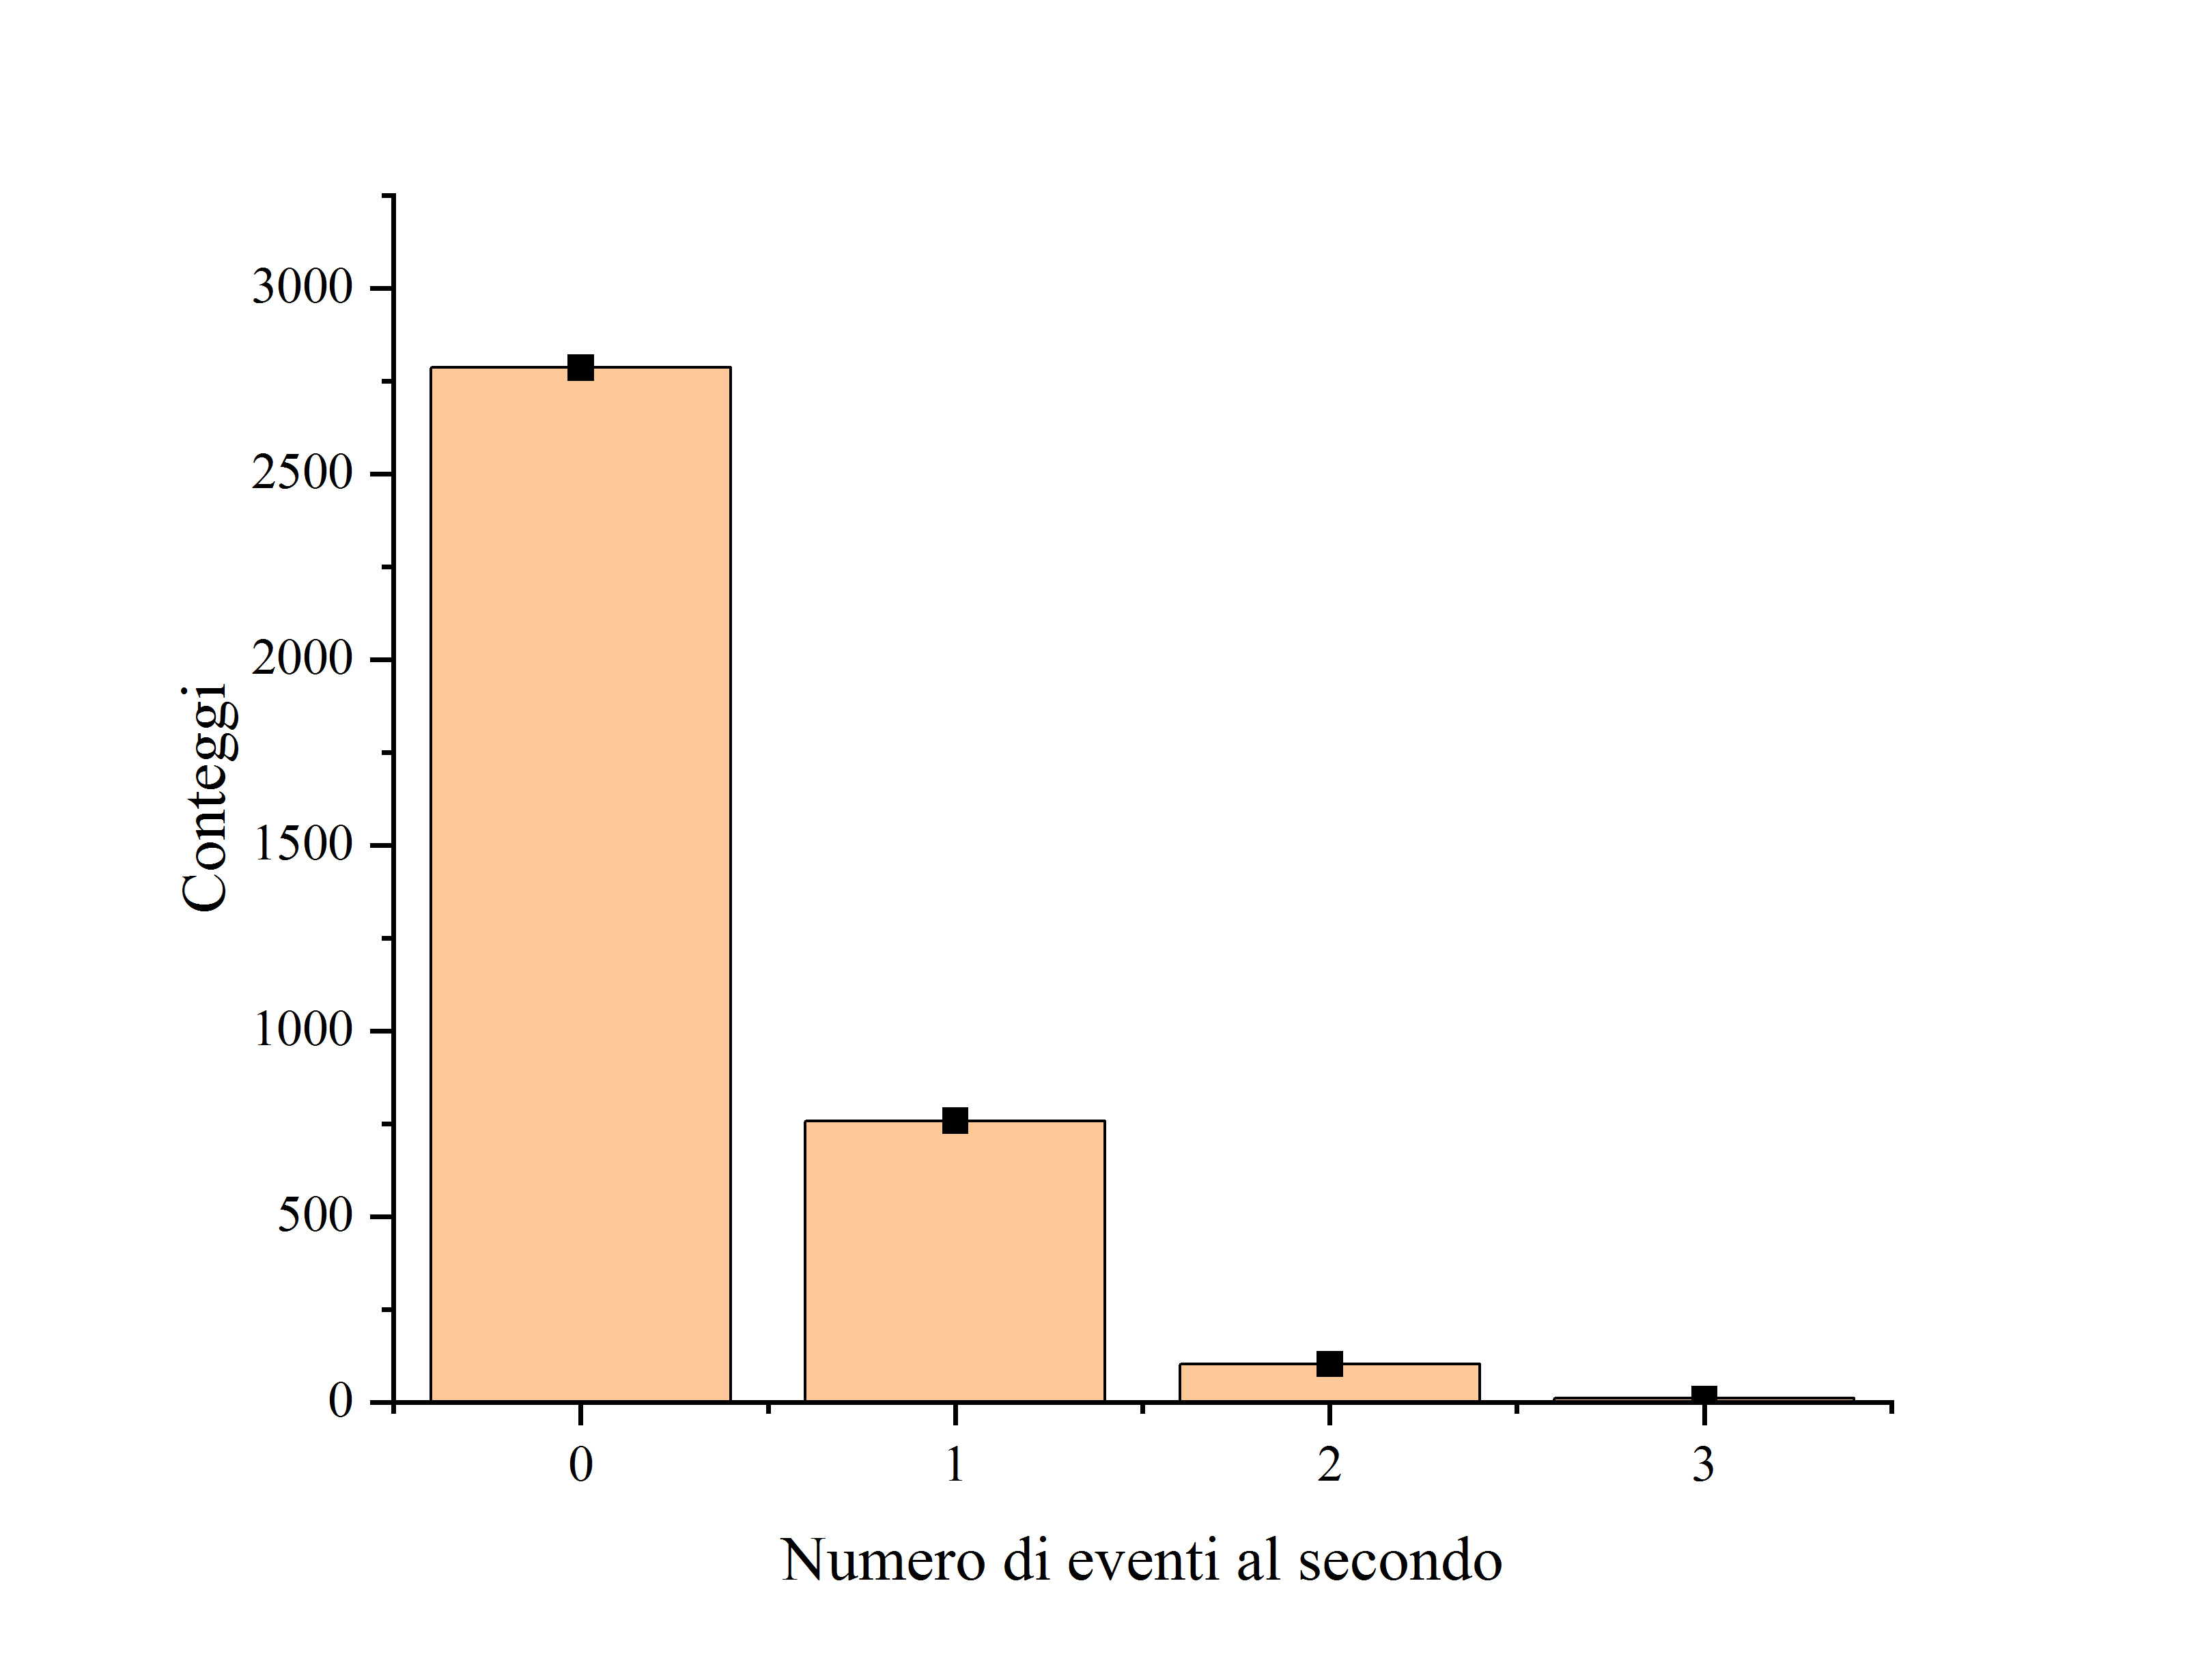
\includegraphics[trim={2cm .5cm 2.4cm 2.1cm},clip,width=.5\textwidth]{img/Geiger4.jpg}
        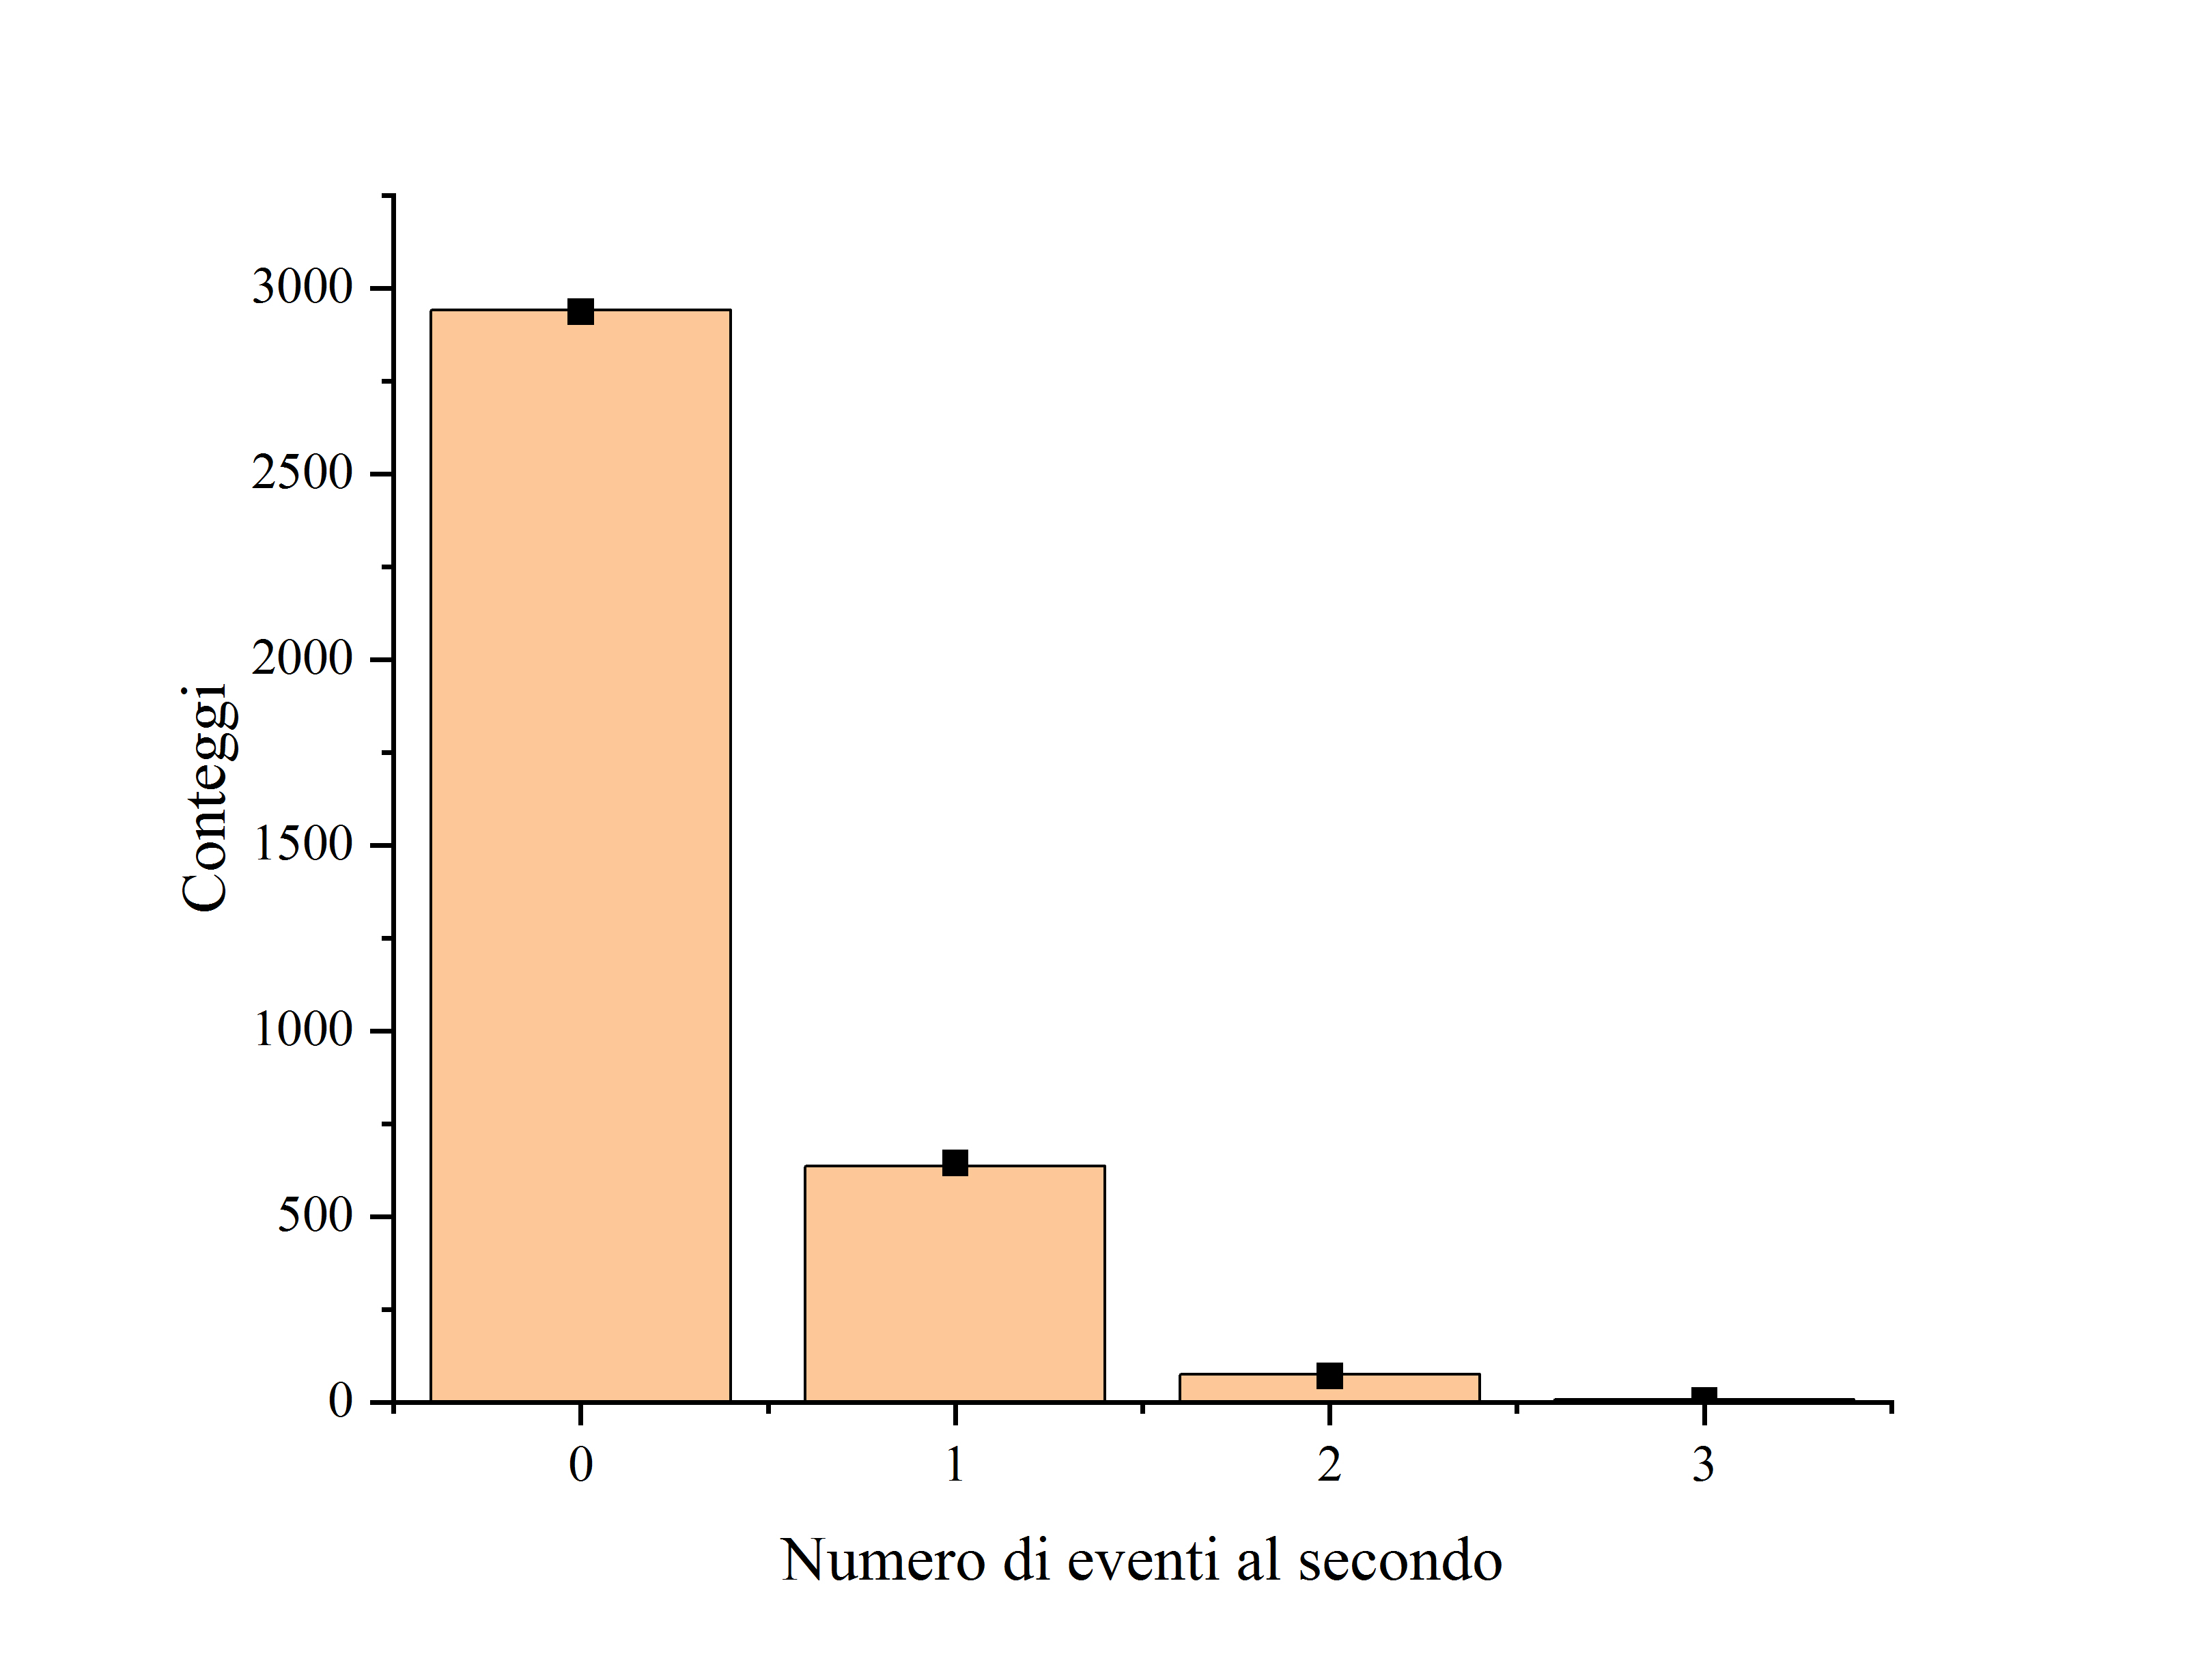
\includegraphics[trim={2cm .5cm 2.4cm 2.1cm},clip,width=.5\textwidth]{img/Geiger5.jpg}
        \caption{Conteggi, nell'ordine, di $x_1$, $x_2$, $x_3$ e $x_4$.}
    \end{figure}
\end{center}

Come si può osservare da questi grafici, i risultati ottenuti si allineano molto bene
alle distribuzioni di Poisson.
Per valutare l'accuratezza della nostra stima di $\overline{x_0}$, possiamo effettuare
una regressione lineare (pesata) utilizzando l'equazione di $x_i$ in funzione di $d_i$:
\[\overline{x_i} = N\xi d_i^{-2} + \overline{x_0}\]
Di seguito riportiamo una tabella con i dati utilizzati per la regressione lineare,
assieme a un grafico della retta di regressione stessa.


\begin{center}
    \begin{tblr}{ |Q[c,m]|Q[c,m]|Q[c,m]|Q[c,m]| }
        \hline
        $i$ & $d_i\;\;(\unit{cm})$ & $d_i^{-2}\;\;(\unit{m^{-2}})$ & $\overline{x_i}$ \\
        \hline
        1 & $9.5\pm0.1$  & $111\pm2$      & $0.809\pm0.015$\\
        2 & $10.3\pm0.1$ & $94.3\pm1.8$   & $0.737\pm0.014$\\
        3 & $26.5\pm0.1$ & $14.24\pm0.11$ & $0.272\pm0.009$\\
        4 & $41.2\pm0.1$ & $5.89\pm0.03$  & $0.219\pm0.008$\\
        \hline
    \end{tblr}
    \begin{figure}[H]
        % trim={< v > ^}
        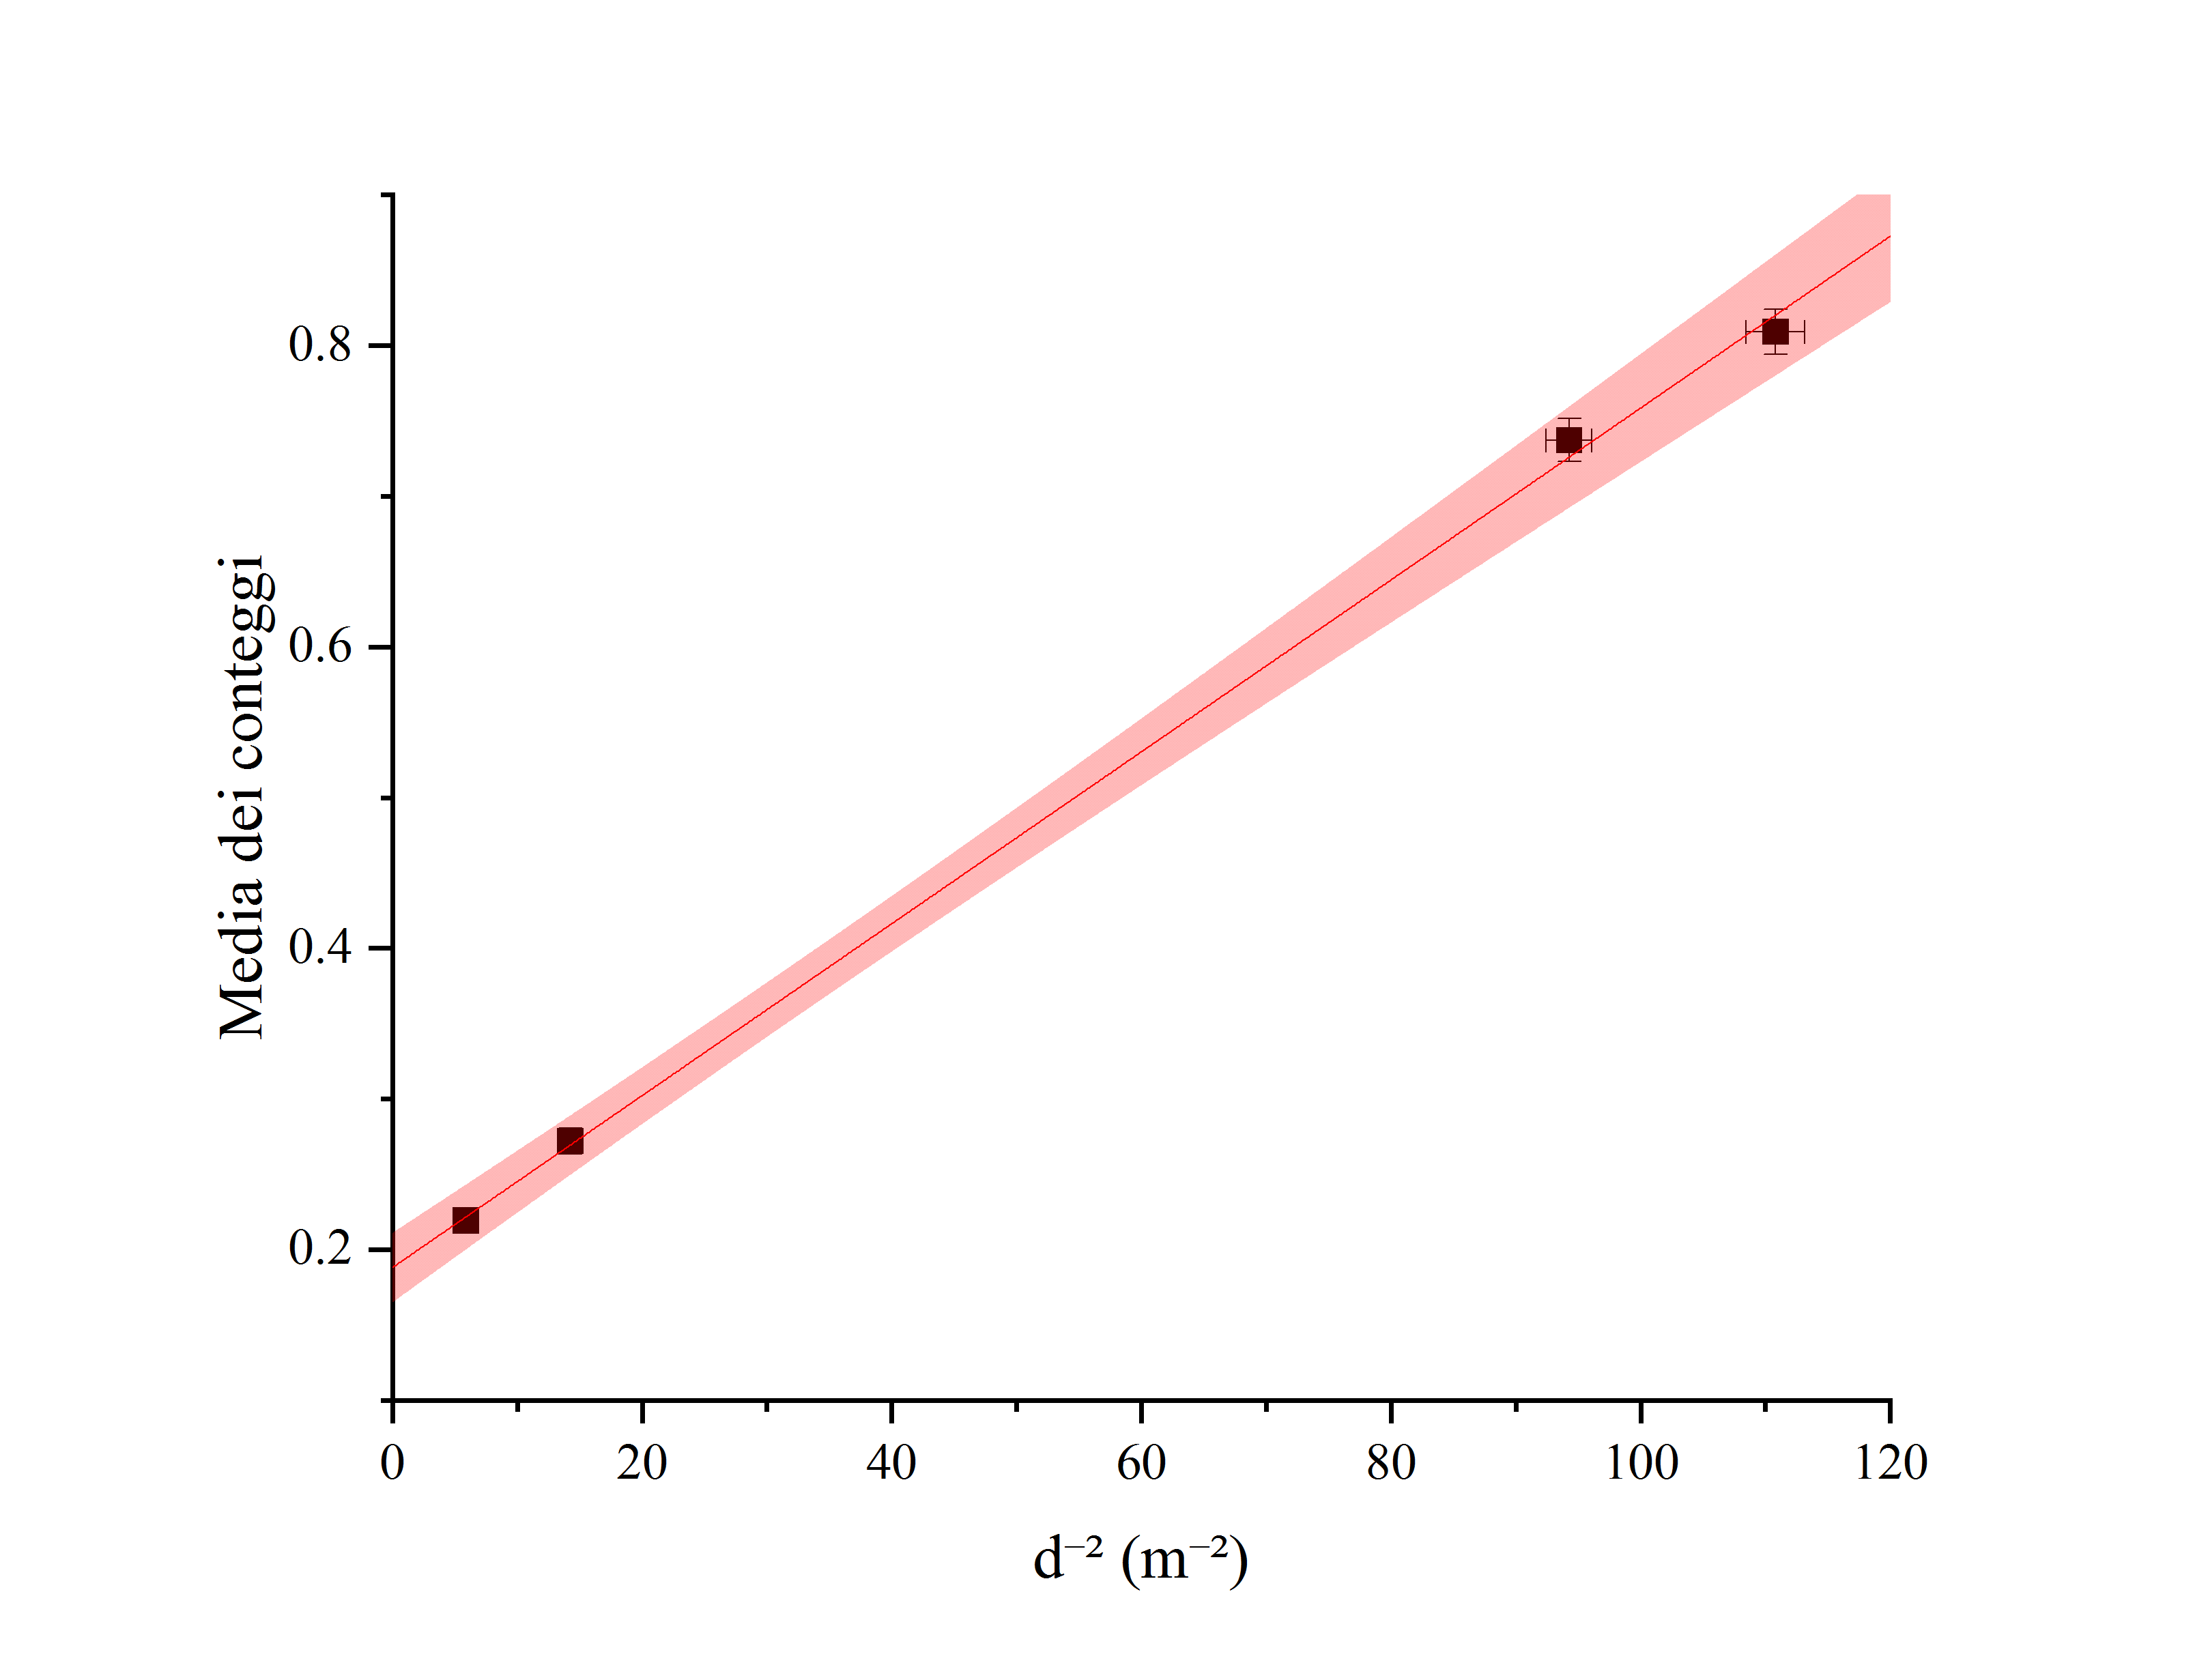
\includegraphics[trim={2cm .5cm 2cm 2.1cm},clip,width=\textwidth]{img/Regressione.png}
        \caption{Regressione lineare. In rosa la regione di incercezza.}
    \end{figure}
\end{center}

Risultati della regressione lineare:
\begin{itemize}
    \item $k$
\end{itemize}

Per valutare numericamente la consistenza tra i due valori di $\overline{x_0}$ ottenuti,
abbiamo calcolato il seguente valore (numero puro):
\[
    \varepsilon =
    \frac{
        \left|\left(k_\text{statica}\right)_\text{best} - \left(k_\text{dinamica}\right)_\text{best}\right|
    }{
        \delta k_\text{statica} + \delta k_\text{dinamica}
    }
\]
Allora $k_\text{statica}$ e $k_\text{dinamica}$ sono consistenti se e solo se $\varepsilon \le 1$.

Nel nostro caso, $\varepsilon = 1.33$. Il gruppo di lavoro ha ipotizzato che
questa inconsistenza (comunque contenuta, seppur non trascurabile) fra le due
misure possa essere ragionevolmente giustificata dalla difficoltà incontrata
nel ridurre al minimo le oscillazioni in direzione perpendicolare a $\vec{g}$;
considerato inoltre che la posizione dei fototraguardi non era ottimale, ciò
potrebbe avere ulteriormente influenzato la distribuzione dei tempi. È in
effetti possibile osservare che le distribuzioni da noi ottenute non sono,
il più delle volte, del tutto simmetriche: la moda sembra essersi spostata
leggermente a sinistra – un possibile sintomo dell'influenza di un
errore sistematico sulle misure.

\pagebreak
\begin{appendices}
    \section{Codice Rust per $10^{12}$ lanci di sei dadi}
    Qui riportiamo il codice Rust, da noi scritto, che ci ha permesso di
    lanciare virtualmente $6\cdot10^{12?}$ dadi in maniera estremamente
    efficiente.

    \inputminted[linenos, mathescape]{rust}{src/main.rs}
\end{appendices}

\end{document}
